\documentclass[11pt,a4paper]{article}

\usepackage[utf8]{inputenc}
\usepackage[margin=1in]{geometry}
\usepackage{amsmath,amssymb,amsfonts,bm}
\usepackage{graphicx}
\graphicspath{{../img/}{./}{img/}}
\usepackage{booktabs}
\usepackage{array}
\usepackage{xcolor}
\usepackage{fancyhdr}
\usepackage{tcolorbox}
\usepackage{listings}
\usepackage{microtype}
\usepackage{hyperref}

% Define palette
\definecolor{primaryblue}{RGB}{24, 76, 120}
\definecolor{secondaryblue}{RGB}{41, 128, 185}
\definecolor{darkgray}{RGB}{44, 62, 80}
\definecolor{lightgray}{RGB}{245, 247, 250}
\definecolor{bordergray}{RGB}{200, 205, 210}
\definecolor{codegreen}{RGB}{39, 174, 96}
\definecolor{codecomment}{RGB}{127, 140, 141}
\definecolor{codekeyword}{RGB}{142, 68, 173}
\definecolor{tunablered}{RGB}{192, 57, 43}

% Hyperref setup
\hypersetup{
    colorlinks=true,
    linkcolor=primaryblue,
    citecolor=primaryblue,
    urlcolor=secondaryblue,
    pdftitle={Lecture 1: AI/ML Foundations and Closed-Loop Control for Particle Accelerators},
    pdfauthor={Chong Shik Park, Ph.D.}
}

% Header and Footer
\pagestyle{fancy}
\fancyhf{}
\fancyhead[L]{\small\color{darkgray}\textbf{AI Applications in Accelerators Tutorial \& Mini-Hackathon}}
\fancyhead[R]{\small\color{darkgray}Lecture Notes}
\fancyfoot[L]{\small\color{darkgray}Lecture 1: AI/ML Foundations \& Closed-Loop Control (Chong Shik Park)}
\fancyfoot[R]{\small\thepage}
\renewcommand{\headrulewidth}{0.6pt}
\renewcommand{\footrulewidth}{0.4pt}

% Affiliation command
\newcommand{\affiliation}[1]{{\normalsize\color{darkgray} #1} \\[0.2em]}

% Code Listing Configuration
\lstdefinestyle{pythonstyle}{
    backgroundcolor=\color{lightgray},
    commentstyle=\color{codecomment}\itshape,
    keywordstyle=\color{codekeyword}\bfseries,
    numberstyle=\tiny\color{codecomment},
    stringstyle=\color{codegreen},
    basicstyle=\ttfamily\footnotesize,
    breakatwhitespace=false,
    breaklines=true,
    captionpos=b,
    keepspaces=true,
    numbers=left,
    numbersep=6pt,
    showspaces=false,
    showstringspaces=false,
    showtabs=false,
    tabsize=4,
    frame=single,
    rulecolor=\color{bordergray}
}
\lstset{style=pythonstyle}

% TColorBox Configuration (Unbreakable boxes kept intact on a single page)
\tcbuselibrary{skins,breakable}
\newtcolorbox{infobox}[1][]{
    enhanced,
    colback=lightgray,
    colframe=primaryblue,
    arc=3mm,
    fonttitle=\bfseries\color{white},
    coltitle=white,
    title=#1,
    left=4mm, right=4mm, top=3mm, bottom=3mm,
    boxrule=0.8pt,
    unbreakable
}

\begin{document}

% Title Banner
\begin{center}
    {\LARGE\bfseries\color{primaryblue} Lecture 1: AI/ML Foundations and Closed-Loop Control for Particle Accelerators} \\[0.8em]
    {\large\color{darkgray} Physics Foundations, Neural Surrogates, Reinforcement Learning, and Bayesian Optimization} \\[0.5em]
    \rule{\textwidth}{1.2pt} \\[0.5em]
    \textbf{Chong Shik Park, Ph.D.} \\[0.3em]
    \affiliation{Department of Accelerator Science, Korea University, Sejong 30019, Republic of Korea}
    \affiliation{Center for Accelerator Research, Korea University, Sejong 30019, Republic of Korea}
    \vspace{0.2em}
    {\small\color{darkgray} November 19, 2026}
\end{center}

\vspace{0.5em}

\begin{abstract}
Modern particle accelerator facilities operate with thousands of tightly coupled magnet actuators and diagnostics under sub-micron beam stability tolerances. Classical linear feedback systems face fundamental bottlenecks in non-linear regimes where magnetic core saturation and power supply limits degrade control fidelity. This lecture provides the theoretical and computational foundation bridging transverse beam dynamics, Hill's equation, and the Orbit Response Matrix (ORM) with cutting-edge supervised machine learning, reinforcement learning, and Bayesian optimization. We explore the design and training of neural surrogate digital twins to model cubic saturation, compare classical singular value decomposition (SVD) with model-based bounded optimization (\texttt{L-BFGS-B}), investigate physics-informed closed-loop reinforcement learning policy agents with adaptive harmonic damping, and examine sample-efficient Bayesian optimization using Gaussian processes and Lower Confidence Bound (LCB) acquisition for the afternoon Beam Orbit Alignment Mini-Hackathon.
\end{abstract}

\clearpage

\tableofcontents

\clearpage

\section{Introduction: AI Applications in Modern Particle Accelerators}

Over the past decade, Artificial Intelligence (AI) and Machine Learning (ML) have evolved from experimental proofs-of-concept into mission-critical operational tools across modern particle accelerator facilities, including synchrotron light sources, free-electron lasers (XFELs), spallation neutron sources, high-intensity hadron linacs, and energy-frontier colliders~\cite{edelen2020opportunities}. Modern accelerators operate with thousands of distributed, non-linearly coupled magnet actuators, radiofrequency (RF) accelerating stations, and high-rate diagnostic monitors under stringent beam quality and stability demands.

The landscape of AI applications in particle accelerators is broadly categorized into five foundational pillars:
\begin{enumerate}
    \item \textbf{Surrogate Modeling \& Fast Digital Twins~\cite{edelen2020opportunities, edelen2018neural}:}
    High-fidelity numerical particle tracking codes (such as \texttt{ELEGANT}, \texttt{MAD-X}, and \texttt{OPAL}) simulate complex beam dynamics, space-charge forces, and collective effects, but require minutes to hours per run. Deep neural networks (Multi-Layer Perceptrons, Convolutional Networks, and Physics-Informed Neural Networks) learn fast surrogate representations capable of evaluating beamline outcomes in sub-millisecond execution times. These ultra-fast surrogates serve as digital twins for real-time model-predictive control, online trajectory correction, and rapid parametric sensitivity analysis.

    \item \textbf{Multi-Objective Autonomous Optimization \& Tuning~\cite{roussel2023turnkey, edelen2020machine}:}
    Commissioning and daily operations involve optimizing conflicting performance objectives---such as maximizing beam transmission and photon brightness while minimizing transverse emittance and beam halo. Bayesian Optimization (BO) with Gaussian Processes, combined with active learning and exploration-exploitation acquisition functions, enables sample-efficient multi-objective optimization directly on physical machines, converging in dozens of shots compared to thousands of iterations required by brute-force parameter scans.

    \item \textbf{Virtual Diagnostics \& Non-Destructive Phase Space Reconstruction~\cite{emma2021virtual}:}
    Critical beam properties---such as 6D phase space, bunch slice emittance, and femtosecond current profiles---often require interceptive diagnostics (e.g., transverse deflection cavities, wire scanners, or screens) that disrupt or destroy the beam. Virtual diagnostics leverage supervised machine learning to accurately reconstruct unmeasured or destructive bunch characteristics shot-by-shot from non-invasive upstream RF probes, magnet currents, and Beam Position Monitor (BPM) signals.

    \item \textbf{Anomaly Detection, Fault Classification \& Machine Protection~\cite{tennant2020supervised}:}
    Unscheduled beam downtime in multi-megawatt hadron linacs and synchrotron facilities incurs heavy scientific and operational costs. Unsupervised machine learning (autoencoders, isolation forests) continuously monitors archival and real-time telemetry to detect subtle precursor drift patterns, while deep sequence models predict high-voltage RF breakdowns, ion source dropouts, and superconducting cavity quenches milliseconds before catastrophic failure, triggering proactive mitigation and machine protection interlocks.

    \item \textbf{Agentic AI \& Autonomous Operation Workflows~\cite{hellert2024autonomous}:}
    Moving beyond single-purpose neural networks, modern research explores autonomous agent architectures (such as \textit{Osprey} and LLM-driven scientific agents). These systems integrate large language models with standardized Python control APIs, simulation engines, and diagnostic databases, enabling high-level natural language operational commands (e.g., ``align the transport line orbit and optimize injection efficiency'') to be autonomously planned, validated, and executed under strict domain guardrails.
\end{enumerate}


\section{Motivation \& Accelerator Physics Foundations}

\subsection{The Operational Stability Challenge}
In synchrotron light sources, free-electron lasers (XFELs), and medical linacs, particle beam stability must be sustained at sub-micron levels to maintain photon brightness and collision luminosity. 

Transverse orbit stability is equally vital in \textbf{hadron linacs} (high-intensity proton and heavy-ion linear accelerators). In modern high-power hadron facilities, uncorrected beam trajectory offsets through accelerating RF cavities and focusing quadrupoles induce strong non-linear space-charge forces, emittance growth, and halo formation. Because high-intensity hadron beams carry enormous beam power, even minute fractional beam losses (exceeding $1\text{ W/m}$ or $10^{-5}$ of total current) induce severe structural radioactivation, prohibiting hands-on maintenance and risking superconducting cavity quenches or vacuum chamber damage.

Orbit distortions arise from multiple sources:
\begin{itemize}
    \item \textbf{Slow Drifts:} Thermal expansion of girders, diurnal ambient temperature shifts, and ground motion.
    \item \textbf{Dynamic Jitter:} Mechanical vibration from cooling water pumps, cryocoolers, and power supply ripple.
    \item \textbf{High Actuator Coupling:} Deflecting a single dipole corrector causes betatron wave propagation across the entire transport line.
\end{itemize}

\subsection{Transverse Beam Dynamics \& Hill's Equation}
In an uncoupled linear transport channel, the transverse displacement $x(s)$ as a function of path length $s$ is governed by \textbf{Hill's Equation}~\cite{wiedemann2015particle}:
\begin{equation}
    \frac{d^2 x(s)}{ds^2} + K(s) x(s) = 0
\end{equation}
where $K(s) = \frac{e}{p} \frac{\partial B_y(s)}{\partial x}$ represents the alternating quadrupole focusing strength ($K > 0$ for horizontal focusing `QF', $K < 0$ for defocusing `QD').

The closed-form betatron solution is given by:
\begin{equation}
    x(s) = \sqrt{\epsilon \beta(s)} \cos\left( \psi(s) + \phi_0 \right)
\end{equation}
where $\beta(s)$ is the Courant-Snyder beta function, $\psi(s) = \int_0^s \frac{d\bar{s}}{\beta(\bar{s})}$ is the betatron phase advance, and $\nu = \frac{1}{2\pi} \oint \frac{ds}{\beta(s)}$ is the betatron tune.

\subsection{Derivation of the Orbit Response Matrix (ORM)}
When an angular kick $\theta_i = \Delta x'_i = \frac{e B L}{p}$ is applied by dipole corrector $i$ at longitudinal position $s_i$, the transverse displacement registered at Beam Position Monitor (BPM) $j$ at position $s_j$ is linearly proportional to the kick angle. (Rows of $\mathbf{R}$ are correctors and columns are BPMs, as in the simulator's \texttt{env.R}.) In a single-pass transport line or linac, which is the hackathon case, only downstream BPMs see the kick, which propagates as a betatron oscillation:
\begin{equation}
    R_{ij} = \frac{\Delta x(s_j)}{\theta_i} = \begin{cases} \sqrt{\beta(s_i)\beta(s_j)}\, \sin\left( \psi(s_j) - \psi(s_i) \right) & (s_j > s_i) \\ 0 & (s_j \le s_i) \end{cases}
\end{equation}
In a circular ring, the kick instead produces a periodic closed-orbit distortion:
\begin{equation}
    R_{ij} = \frac{\sqrt{\beta(s_i)\beta(s_j)}}{2 \sin(\pi \nu)} \cos\left( |\psi(s_j) - \psi(s_i)| - \pi \nu \right)
\end{equation}
The hackathon simulator models the single-pass transport line using simplified betatron optics with a constant phase advance of $2\pi \cdot 0.18\text{ rad/m}$ and a slowly decaying amplitude:
\begin{equation}
    R_{ij} = \frac{1.2\,\sin\left(2\pi \cdot 0.18\,(s_j - s_i)\right)}{1 + 0.05\,(s_j - s_i)}, \qquad (s_j > s_i)
\end{equation}
For $M$ BPMs and $N$ dipole steerers, the linear response is encapsulated by the matrix $\mathbf{R} \in \mathbb{R}^{N \times M}$~\cite{minty2003measurement}:
\begin{equation}
    \mathbf{Y}_{\text{linear}} = \mathbf{I} \cdot \mathbf{R}
\end{equation}
where $\mathbf{I} = [I_1, I_2, \dots, I_N]$ represents the corrector current vector.

\begin{figure}[t!]
\centering
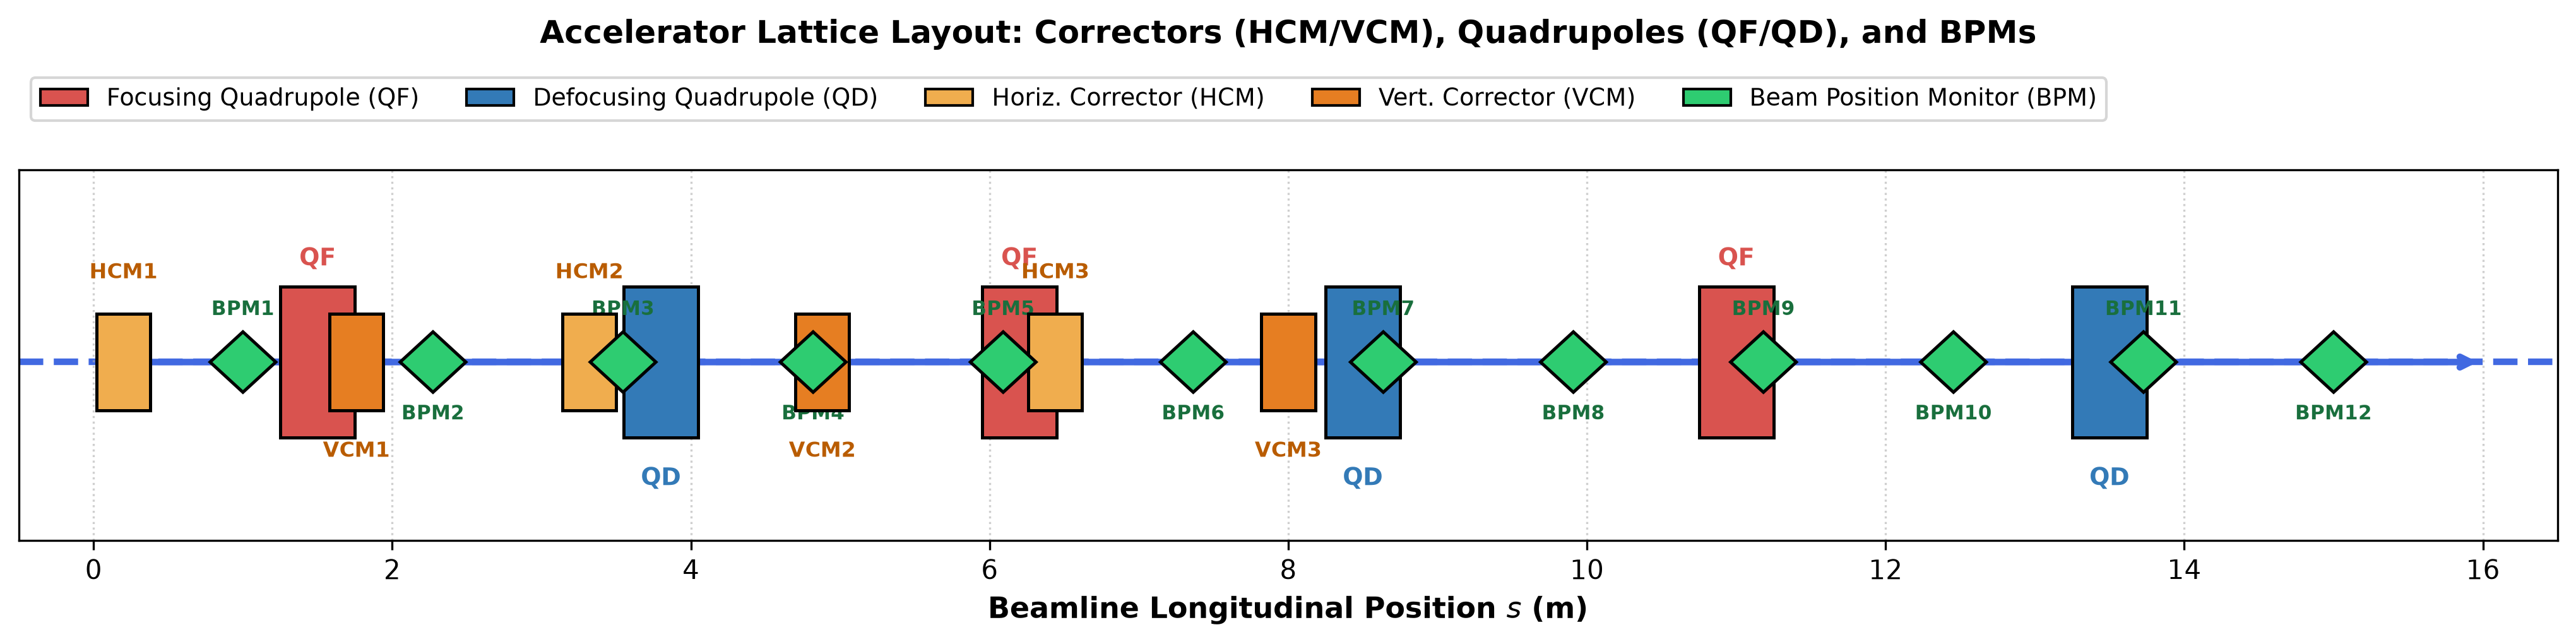
\includegraphics[width=0.95\textwidth]{beamline.png}
\caption{Schematic diagram of the 15-meter accelerator transport section showing alternating focusing (QF, red) and defocusing (QD, blue) quadrupoles, 6 dipole steerers (HCM/VCM), and 12 Beam Position Monitors.}
\label{fig:beamline}
\end{figure}

\subsection{Mini-Hackathon Lattice Geometry \& Realistic Non-Linearities}
The mini-hackathon benchmark lattice (Figure~\ref{fig:beamline}) models a 15-meter transport line:
\begin{itemize}
    \item \textbf{Actuators:} 6 dipole steerers (3 Horizontal `HCM1--3', 3 Vertical `VCM1--3') bounded in $[-5.0\text{ A}, +5.0\text{ A}]$, with single-step adjustments clipped to $[-0.8\text{ A}, +0.8\text{ A}]$.
    \item \textbf{Diagnostics:} 12 Beam Position Monitors ($s = 1.0\text{ m}$ to $15.0\text{ m}$) reading beam displacement in millimeters.
    \item \textbf{Magnetic Core Saturation:} Ferromagnetic saturation at higher excitation currents induces non-linear cubic rolloff:
    \begin{equation}
        \mathbf{Y}_{\text{sat}} = - 0.015 \cdot (\mathbf{I}^3 \cdot \mathbf{R})
    \end{equation}
    \item \textbf{Initial Orbit Distortion ($\mathbf{Y}_0$):} Steering and alignment errors upstream of the line produce an initial orbit distortion that the controller does not know in advance. The simulator models it as unknown steering kicks at all six corrector locations, $\mathbf{Y}_0 = \mathbf{a} \cdot \mathbf{R}$ with $a_k \sim \mathcal{U}(-2.5, 2.5)\text{ A}$ drawn for each episode seed, giving initial RMS errors of $0.93$--$3.59\text{ mm}$ on the 30 evaluation seeds. Because the distortion lies in the span of the corrector responses, a perfect controller can cancel it down to the sensor noise, but this needs total currents up to about $2.8\text{ A}$, where the cubic saturation softens the magnets by up to 12\%, and about 3 to 4 steps of at most $0.8\text{ A}$.
    \item \textbf{Gaussian Measurement Noise:} Sensor electronics introduce random noise $\boldsymbol{\epsilon} \sim \mathcal{N}(0, \sigma^2)$, with $\sigma = 0.010\text{ mm}$ ($10\ \mu\text{m}$).
\end{itemize}

The complete physical forward response equation is:
\begin{equation}
    \mathbf{Y} = \mathbf{I} \cdot \mathbf{R} - 0.015 \cdot (\mathbf{I}^3 \cdot \mathbf{R}) + \mathbf{Y}_0 + \boldsymbol{\epsilon}
\end{equation}


\section{Machine Learning Fundamentals \& Neural Surrogate Modeling}

\subsection{Machine Learning Taxonomy in Accelerators}
Machine Learning (ML) algorithms automatically extract functional mappings from numerical tracking simulations or machine archives without requiring explicit analytical re-derivation. In accelerator operations, ML encompasses three main paradigms:
\begin{itemize}
    \item \textbf{Supervised Learning:} Learning a continuous regression mapping $\mathbf{Y} = f(\mathbf{X})$ from actuator magnet currents $\mathbf{X}$ to beam diagnostic offsets $\mathbf{Y}$. This forms the foundation of \textbf{Surrogate Modeling / Digital Twins}.
    \item \textbf{Unsupervised Learning:} Uncovering latent structures in unlabelled data (e.g., PCA for betatron mode decomposition, autoencoders for anomaly detection).
    \item \textbf{Reinforcement Learning (RL):} Training an agent policy $\pi(a|s)$ through environmental interaction to maximize cumulative reward for \textbf{Autonomous Closed-Loop Control}.
\end{itemize}

\subsection{Foundational ML Paradigms: Forward Supervised Learning vs. Reinforcement Learning}
In developing autonomous beam alignment algorithms, accelerator engineers rely primarily on two complementary paradigms: \textbf{Forward Supervised Learning} (training a digital twin surrogate of the accelerator to be inverted) and \textbf{Reinforcement Learning} (training a closed-loop policy agent that directly interacts with the machine). Figure~\ref{fig:sl_vs_rl} illustrates their distinct architectural workflows.

\begin{figure}[t!]
\centering
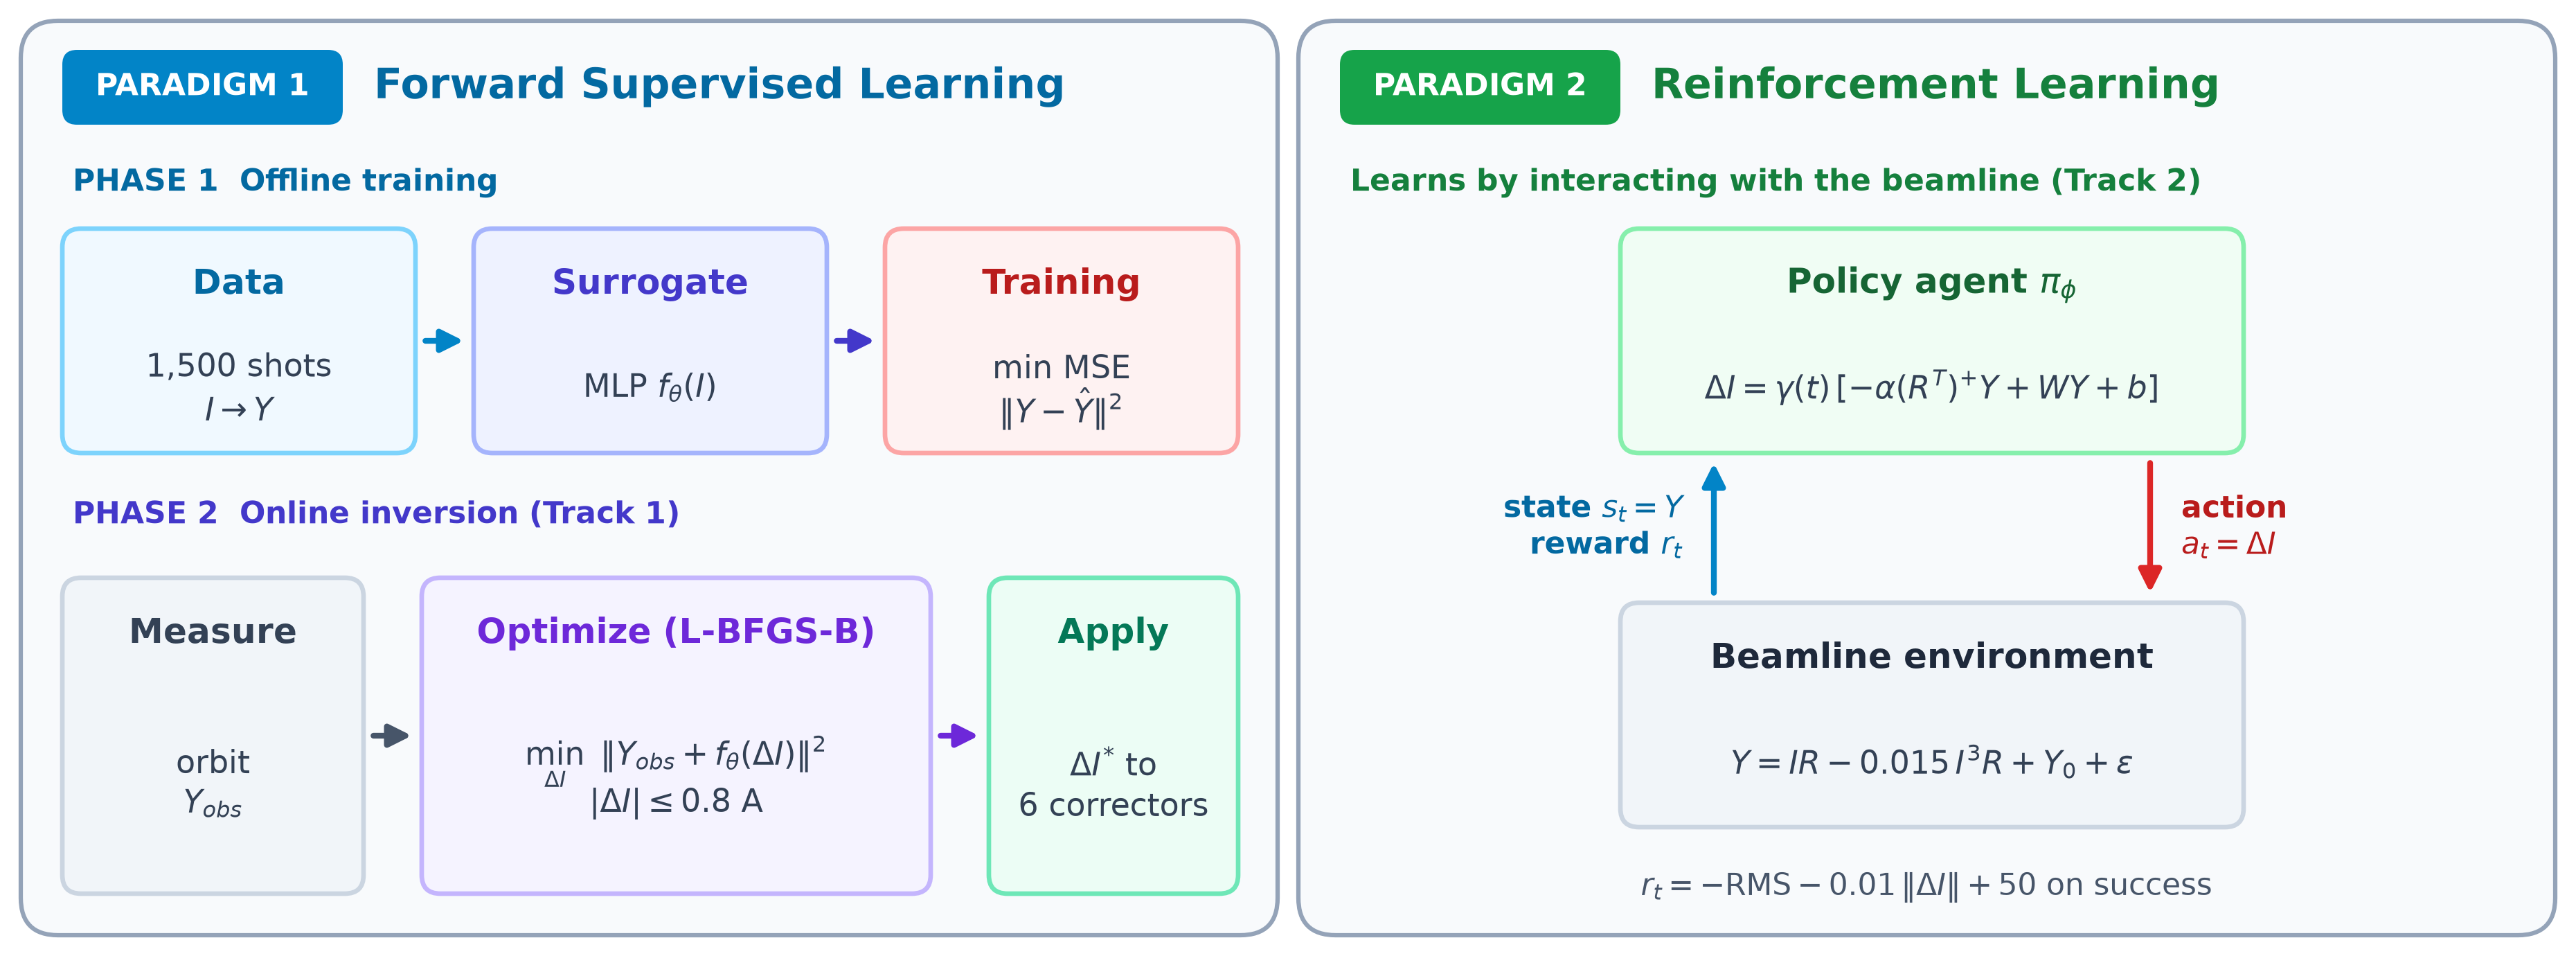
\includegraphics[width=0.98\textwidth]{forward_sl_and_rl_schematic.png}
\caption{The three learning paradigms behind the challenge tracks: supervised surrogate learning with online inversion (Track~1), reinforcement learning by interaction with the beamline (Track~2), and Bayesian optimization with a Gaussian process model and its uncertainty (Track~3), whose GP can optionally be refit online.}
\label{fig:sl_vs_rl}
\end{figure}

\subsubsection{Forward Supervised Learning: Digital Twin Surrogate \& Inversion (Track 1)}
In Forward Supervised Learning, the model learns the predictive forward response mapping $\mathbf{I} \mapsto \mathbf{Y}$ from passive, pre-recorded tracking simulation datasets:
\begin{enumerate}
    \item \textbf{Offline Dataset Generation:} We sample $N$ random corrector current vectors $\mathbf{I} \in \mathbb{R}^6$ across operating ranges (e.g., $[-3.0\text{ A}, +3.0\text{ A}]$) and evaluate their transverse displacements $\mathbf{Y} \in \mathbb{R}^{12}$ across all 12 BPMs, yielding dataset $\mathcal{D} = \{(\mathbf{I}^{(i)}, \mathbf{Y}^{(i)})\}_{i=1}^N$.
    \item \textbf{Surrogate Model Training:} A deep neural network (e.g. Multi-Layer Perceptron $f_{\boldsymbol{\theta}}$ with layers $128 \rightarrow 64 \rightarrow 32$) is trained to minimize the Mean Squared Error (MSE) loss:
    \begin{equation}
        \mathcal{L}_{\text{MSE}}(\boldsymbol{\theta}) = \frac{1}{N} \sum_{i=1}^N \left\| \mathbf{Y}^{(i)} - f_{\boldsymbol{\theta}}(\mathbf{I}^{(i)}) \right\|_2^2
    \end{equation}
    A well-trained surrogate captures the non-linear magnetic core saturation $B(I) \approx I - 0.015 \cdot I^3$ down to the $0.010\text{ mm}$ diagnostic noise floor.
    \item \textbf{Online Inversion for Beam Alignment:} During beam operations, observed orbit distortions $\mathbf{Y}_{\text{obs}}$ are corrected by solving an online bounded minimization problem:
    \begin{equation}
        \Delta \mathbf{I}^* = \arg\min_{\Delta \mathbf{I}} \left\| \mathbf{Y}_{\text{obs}} - f_{\boldsymbol{\theta}}(\mathbf{I}) + f_{\boldsymbol{\theta}}(\mathbf{I} + \Delta \mathbf{I}) \right\|_2^2 + \lambda \|\Delta \mathbf{I}\|_2^2
    \end{equation}
    subject to hardware delta limits $\Delta \mathbf{I} \in [-0.8\text{ A}, +0.8\text{ A}]^6$. Because the surrogate captures soft saturation, this approach converges in as few as 2 to 3 iterations.
\end{enumerate}

\subsubsection{Reinforcement Learning: Closed-Loop Policy Control (Track 2)}
In Reinforcement Learning (RL), orbit steering is formulated as a Markov Decision Process (MDP) $(\mathcal{S}, \mathcal{A}, \mathcal{P}, \mathcal{R}, \gamma)$:
\begin{enumerate}
    \item \textbf{State Space ($\mathcal{S}$):} Transverse beam offsets measured at 12 BPM stations: $\mathbf{s}_t = \mathbf{Y}_t \in [-10.0\text{ mm}, +10.0\text{ mm}]^{12}$.
    \item \textbf{Action Space ($\mathcal{A}$):} Corrector kick delta currents: $\mathbf{a}_t = \Delta \mathbf{I}_t \in [-0.8\text{ A}, +0.8\text{ A}]^6$.
    \item \textbf{Environment Dynamics ($\mathcal{P}$):} Physical transport law including betatron optics, core saturation, the initial steering-error distortion $\mathbf{Y}_0$, and sensor noise $\boldsymbol{\epsilon}$:
    \begin{equation}
        \mathbf{I}_{t+1} = \text{clip}(\mathbf{I}_t + \mathbf{a}_t, -5.0, +5.0)\text{ A}, \quad \mathbf{s}_{t+1} = \mathbf{I}_{t+1} \cdot \mathbf{R} - 0.015 \cdot (\mathbf{I}_{t+1}^3 \cdot \mathbf{R}) + \mathbf{Y}_0 + \boldsymbol{\epsilon}
    \end{equation}
    \item \textbf{Reward Signal ($\mathcal{R}$):} Scalar feedback rewarding alignment precision and penalizing actuator effort and steps:
    \begin{equation}
        r_t = - w_{\text{rms}} \cdot \text{RMS}_{t+1} - w_{\text{act}} \cdot \|\mathbf{a}_t\|_2^2 - c_{\text{step}} + (B_{\text{success}} \text{ if terminated else } 0.0)
    \end{equation}
    \item \textbf{Physics-Informed Prior \& Adaptive Damping:} High-performance policies synthesize an analytical pseudo-inverse prior with learned non-linear residual compensation and dynamic step cooling:
    \begin{equation}
        \Delta \mathbf{I}_t = \gamma(t) \cdot \left[ - \alpha (\mathbf{R}^T)^\dagger \mathbf{Y}_t + \mathbf{W}_{\text{learned}} \mathbf{Y}_t + \mathbf{b} \right], \quad \gamma(t) = \frac{1.0}{1.0 + 0.03 \cdot t}
    \end{equation}
    The policy is evaluated in a single forward pass: about $0.01\text{ ms}$ per step for the reference agent, against about $27\text{ ms}$ for per-step surrogate inversion.
\end{enumerate}

\subsubsection{Comparative Architectural Analysis}
Table~\ref{tab:sl_vs_rl} summarizes the fundamental operational differences between the two paradigms.

\begin{table}[h!]
\centering
\small
\begin{tabular}{p{3.5cm} p{5.5cm} p{5.5cm}}
\toprule
\textbf{Dimension} & \textbf{Forward Supervised Learning (Track 1)} & \textbf{Reinforcement Learning (Track 2)} \\
\midrule
\textbf{Primary Goal} & Accurate physical predictive twin ($\hat{\mathbf{Y}} = f_{\boldsymbol{\theta}}(\mathbf{I})$) & Optimal closed-loop action policy ($\mathbf{a}_t = \pi_{\boldsymbol{\phi}}(\mathbf{s}_t)$) \\
\textbf{Data Source} & Offline passive sampling across grid & Online interactive rollouts in environment \\
\textbf{Training Signal} & Ground-truth diagnostic vectors $\mathbf{Y}$ & Scalar reward feedback $r_t$ \\
\textbf{Objective} & Minimize MSE / RMSE error & Maximize cumulative return $\mathbb{E}[\sum \gamma^t r_t]$ \\
\textbf{Control Mechanism} & Forward twin + SciPy \texttt{L-BFGS-B} solver & Direct feedback policy evaluation \\
\textbf{Execution Latency} & About $27\text{ ms}$ per step & About $0.01\text{ ms}$ per step \\
\textbf{Sample Efficiency} & High ($1,500$ shots trains full model) & Moderate to high (with physics priors) \\
\textbf{Safety Handling} & Explicit box constraints in optimizer & Hardware action clipping \& damping \\
\bottomrule
\end{tabular}
\caption{Comparison of Forward Supervised Learning vs.\ Closed-Loop Reinforcement Learning for accelerator control.}
\label{tab:sl_vs_rl}
\end{table}

\subsection{Model Training Terminology \& Operational Definitions}
To systematically design, train, and diagnose neural network models in accelerator physics, engineers must master the standard mathematical and operational terminology of model training:

\begin{enumerate}
    \item \textbf{Weights ($\mathbf{W}$) \& Biases ($\mathbf{b}$):}
    \begin{itemize}
        \item \textbf{Weights ($\mathbf{W} \in \mathbb{R}^{m \times n}$):} Trainable synaptic scaling multipliers that weight the contribution of input features or upstream activations. In beam physics surrogates, weights encode the effective transport coupling between magnetic fields and trajectory deflections.
        \item \textbf{Biases ($\mathbf{b} \in \mathbb{R}^m$):} Trainable affine translation vectors that shift the activation threshold of a neuron independently of the inputs, allowing the network to represent non-zero baselines (e.g., unsteered closed-orbit distortion offsets $\mathbf{Y}_0$).
    \end{itemize}

    \item \textbf{Activation Functions ($\sigma(z)$) and their Four Essential Operational Roles:}
    An activation function $\sigma: \mathbb{R} \to \mathbb{R}$ is a non-linear operator applied element-wise to pre-activation affine sums $z = \mathbf{w}^T \mathbf{x} + b$. In accelerator surrogate modeling, activation functions fulfill four critical roles:
    \begin{itemize}
        \item \textbf{Role 1: Breaking Linearity (Preventing Model Collapse):} Without non-linear activations, stacking $L$ sequential dense layers mathematically collapses into a single matrix product $\mathbf{W}_{\text{eff}} = \mathbf{W}^{(L)} \cdots \mathbf{W}^{(1)}$, rendering a deep network no more expressive than a linear Orbit Response Matrix (ORM).
        \item \textbf{Role 2: Universal Approximation of Non-Linear Physical Dynamics:} By introducing non-linearities, neural networks become universal function approximators (Hornik et al., 1989), allowing them to capture non-linear accelerator phenomena such as iron-core saturation $B(I) \propto I - 0.015 I^3$, sextupole fields, and chromatic aberrations.
        \item \textbf{Role 3: Gating Backpropagation Gradients:} The derivative $\sigma'(z)$ acts as a transmission gate for error gradients during backpropagation. Non-saturating activations (such as ReLU with $\sigma'(z) = 1$ for $z > 0$) prevent gradients from vanishing across deep layers, ensuring stable gradient descent.
        \item \textbf{Role 4: Enforcing Physical Output Bounds:} Selecting the appropriate activation function ensures output values conform to physical reality. While intermediate hidden layers require non-linearities, output regression layers predicting unconstrained spatial coordinates ($mm$) must strictly use linear identity activations to avoid artificial truncation.
    \end{itemize}

    \item \textbf{Loss Functions ($\mathcal{L}$) and Loss Rates:}
    A scalar objective measuring discrepancy between model predictions $\hat{\mathbf{Y}} = f_{\boldsymbol{\theta}}(\mathbf{X})$ and physical ground truth $\mathbf{Y}$. In regression surrogates, Mean Squared Error (MSE) is standard:
    \begin{equation}
        \mathcal{L}_{\text{MSE}}(\boldsymbol{\theta}) = \frac{1}{N \cdot M} \sum_{i=1}^N \sum_{j=1}^M \left( Y_{i,j} - \hat{Y}_{i,j}(\boldsymbol{\theta}) \right)^2
    \end{equation}
    The loss rate ($\Delta \mathcal{L} / \Delta \text{epoch}$) is steep initially as linear optics components are fitted, then flattens as subtle non-linearities are resolved down to the sensor noise floor ($\sigma = 10\ \mu\text{m}$).

    \item \textbf{Gradients ($\nabla_{\boldsymbol{\theta}}\mathcal{L}$) and Backpropagation:}
    The gradient vector $\nabla_{\boldsymbol{\theta}}\mathcal{L}$ points in the direction of steepest loss ascent. Backpropagation applies the multivariable chain rule recursively from output to input, evaluating exact parameter gradients in $O(|\boldsymbol{\theta}|)$ time rather than costly finite differences.

    \item \textbf{Epoch, Batch Size ($B$), and Step / Iteration:}
    \begin{itemize}
        \item \textbf{Epoch:} Exactly one complete pass through the entire training dataset ($N$ shots).
        \item \textbf{Batch Size ($B$):} The number of training samples processed in parallel before performing a parameter update. Mini-batching ($B \in [32, 128]$) provides stochastic regularization against sensor jitter.
        \item \textbf{Step / Iteration:} A single parameter update $\boldsymbol{\theta} \leftarrow \boldsymbol{\theta} - \Delta \boldsymbol{\theta}$. An epoch contains $\lceil N / B \rceil$ steps.
    \end{itemize}

    \item \textbf{Learning Rate ($\eta$) \& Optimization Schedules:}
    The scalar hyperparameter scaling parameter updates: $\boldsymbol{\theta}_{t+1} = \boldsymbol{\theta}_t - \eta \cdot \mathbf{g}_t$. Excessively large $\eta$ causes numerical divergence; excessively small $\eta$ causes glacial convergence. Schedulers dynamically reduce $\eta$ as the model approaches optimal convergence.

    \item \textbf{Regularization ($L_2$ Weight Decay, Early Stopping):}
    \begin{itemize}
        \item \textbf{$L_2$ Regularization ($\alpha$):} Adds penalty $\frac{1}{2}\alpha \|\mathbf{W}\|_2^2$ to the loss, suppressing overfitting to Gaussian diagnostic jitter ($\boldsymbol{\epsilon} \sim 10\ \mu\text{m}$).
        \item \textbf{Early Stopping:} Monitors validation loss on a separate holdout split; terminates training when validation loss stops improving to preserve optimal generalization.
    \end{itemize}

    \item \textbf{Generalization, Overfitting vs.\ Underfitting:}
    Underfitting (high bias) occurs when the model is too simple to represent physical non-linearities (e.g. linear ORM on saturated magnets). Overfitting (high variance) occurs when excess capacity memorizes measurement noise. Generalization reflects accurate trajectory prediction on unseen machine states.
\end{enumerate}

\subsection{Activation Functions Catalog: Mathematics, Gradients, and Selection}
The choice of activation function directly determines the non-linear expressive capacity and training stability of accelerator neural networks (Figure~\ref{fig:activations}):

\begin{figure}[h!]
\centering
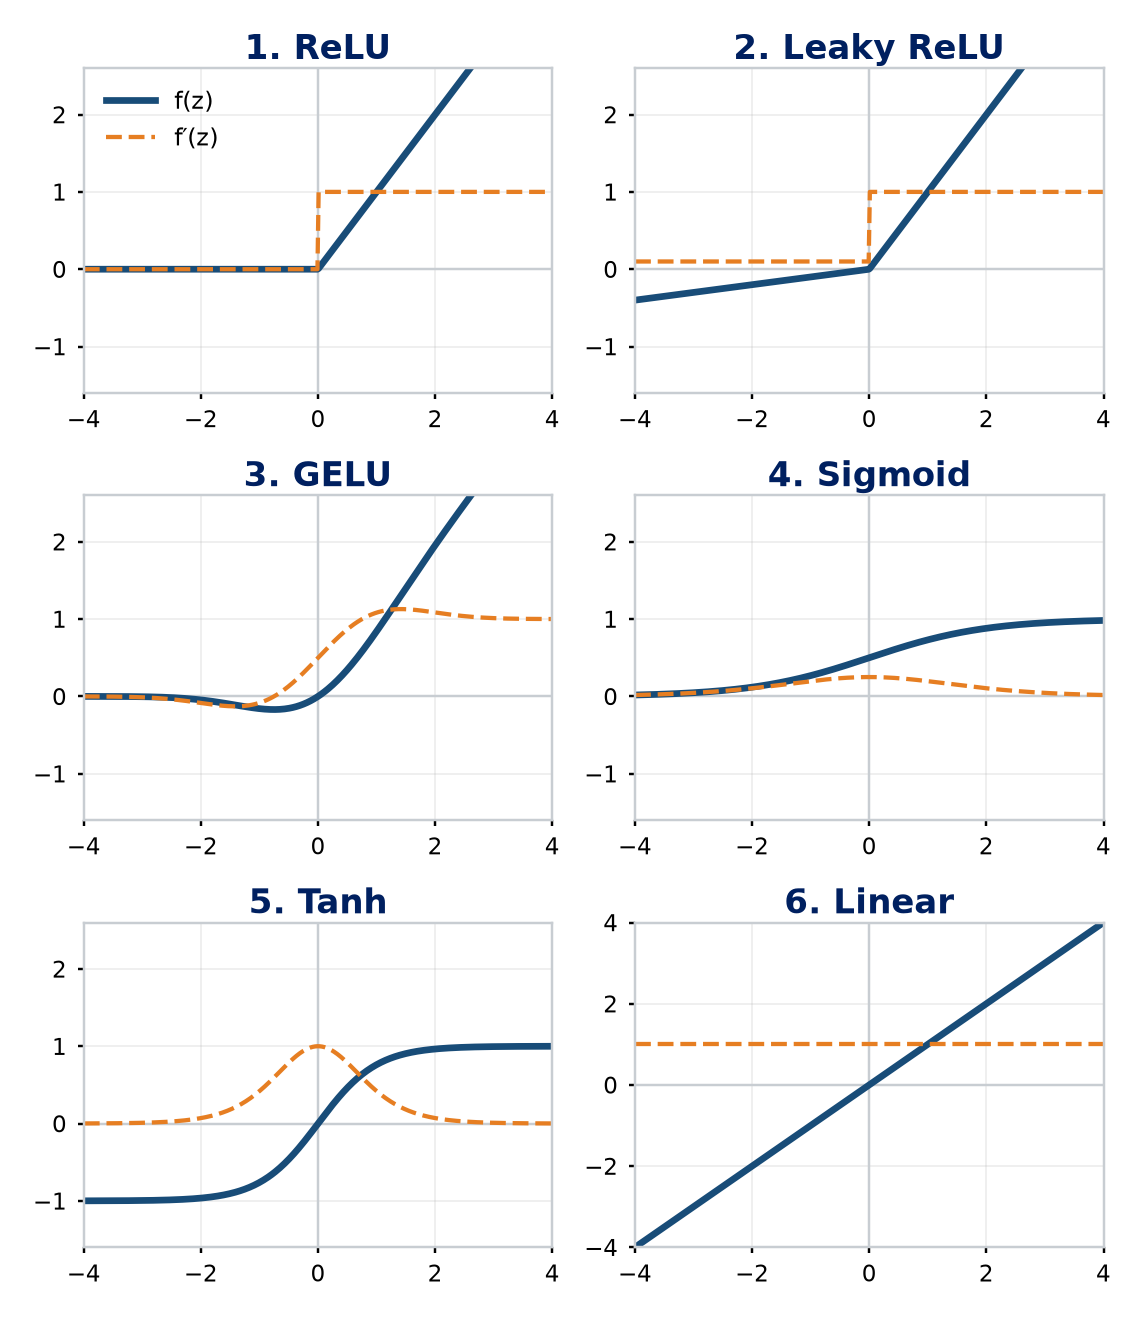
\includegraphics[width=0.62\textwidth]{activation_functions.png}
\caption{Six common activation functions $f(z)$ (solid) and their gradients $f'(z)$ (dashed). Sigmoid and Tanh gradients vanish for large $|z|$, while ReLU keeps a constant gradient for $z > 0$.}
\label{fig:activations}
\end{figure}

\begin{enumerate}
    \item \textbf{Rectified Linear Unit (ReLU):}
    \begin{equation}
        f(z) = \max(0, z), \qquad f'(z) = \begin{cases} 1 & \text{if } z > 0 \\ 0 & \text{if } z < 0 \end{cases}
    \end{equation}
    Gradient is strictly 1.0 for positive activations, eliminating vanishing gradients. Evaluated via a single conditional instruction.
    \item \textbf{Leaky ReLU:}
    \begin{equation}
        f(z) = \max(\alpha z, z), \quad \alpha \approx 0.01, \qquad f'(z) = \begin{cases} 1 & \text{if } z > 0 \\ \alpha & \text{if } z \le 0 \end{cases}
    \end{equation}
    Provides a small slope $\alpha$ for negative arguments, preventing ``dying'' neurons from permanently deactivating.
    \item \textbf{Gaussian Error Linear Unit (GELU):}
    \begin{equation}
        f(z) = z \cdot \Phi(z) = z \cdot \frac{1}{2}\left[1 + \text{erf}\left(\frac{z}{\sqrt{2}}\right)\right]
    \end{equation}
    Smooth probabilistic gating based on the standard normal CDF, standard in modern Transformers.
    \item \textbf{Sigmoid:}
    \begin{equation}
        \sigma(z) = \frac{1}{1 + e^{-z}}, \qquad \sigma'(z) = \sigma(z)(1 - \sigma(z))
    \end{equation}
    Smoothly bounds outputs to $(0, 1)$, but gradients vanish severely for $|z| > 4$.
    \item \textbf{Hyperbolic Tangent ($\tanh$):}
    \begin{equation}
        \tanh(z) = \frac{e^z - e^{-z}}{e^z + e^{-z}}, \qquad \tanh'(z) = 1 - \tanh^2(z)
    \end{equation}
    Zero-centered in $(-1, 1)$. Near the origin, $\tanh(z) \approx z$, effective for modeling smooth linear perturbations with gentle saturation.
    \item \textbf{Linear / Identity:} $f(z) = z$, $f'(z) = 1$. Strictly required for the output regression layer to avoid unphysical coordinate clipping.
\end{enumerate}

\subsection{Worked Example: Neural Surrogate for a Particle Transfer Matrix}
To bridge deep learning directly with accelerator beam physics, consider surrogating a linear beamline section characterized by a particle transfer matrix. The companion notebook \texttt{notebooks/Transfer\_Matrix\_Surrogate\_Phase\_Space.ipynb} trains this network for a FODO cell and compares it with the matrix in phase space.

\subsubsection{Classical Analytical Transfer Matrix Formulation}
In linear beam optics, the transverse phase-space trajectory of a particle from initial position $s_0$ to final diagnostic station $s_f$ is governed by the $2 \times 2$ transfer matrix $\mathbf{M}$:
\begin{equation}
    \begin{pmatrix} x_f \\ x'_f \end{pmatrix} = \mathbf{M} \begin{pmatrix} x_0 \\ x'_0 \end{pmatrix} = \begin{pmatrix} C(s) & S(s) \\ C'(s) & S'(s) \end{pmatrix} \begin{pmatrix} x_0 \\ x'_0 \end{pmatrix}
\end{equation}
where $x$ is the transverse offset ($mm$), $x' = dx/ds$ is the angle ($mrad$), and the determinant satisfies the symplectic condition (Liouville's theorem / phase-space area conservation):
\begin{equation}
    \det \mathbf{M} = C(s)S'(s) - S(s)C'(s) \equiv 1
\end{equation}
Under unperturbed transport, a matched beam ellipse $\gamma x^2 + 2\alpha x x' + \beta x'^2 = \epsilon$ maps into another ellipse of identical invariant area $\pi \epsilon$.

\subsubsection{Neural Network Surrogate Architecture}
We construct a neural surrogate $f_{\boldsymbol{\theta}}: \mathbb{R}^2 \to \mathbb{R}^2$ that ingests initial coordinates $(x_0, x'_0)$ and predicts final coordinates $(\hat{x}_f, \hat{x}'_f)$:
\begin{equation}
    \begin{pmatrix} \hat{x}_f \\ \hat{x}'_f \end{pmatrix} = f_{\boldsymbol{\theta}}\begin{pmatrix} x_0 \\ x'_0 \end{pmatrix} = \mathbf{W}^{(3)} \sigma\left( \mathbf{W}^{(2)} \sigma\left( \mathbf{W}^{(1)} \begin{pmatrix} x_0 \\ x'_0 \end{pmatrix} + \mathbf{b}^{(1)} \right) + \mathbf{b}^{(2)} \right) + \mathbf{b}^{(3)}
\end{equation}
Trained over $N$ tracking pairs $\mathcal{D} = \{((x_{0,i}, x'_{0,i}), (x_{f,i}, x'_{f,i}))\}_{i=1}^N$ using Mean Squared Error loss:
\begin{equation}
    \mathcal{L}_{\text{MSE}}(\boldsymbol{\theta}) = \frac{1}{N} \sum_{i=1}^N \left[ \left( x_{f,i} - \hat{x}_{f,i} \right)^2 + \left( x'_{f,i} - \hat{x}'_{f,i} \right)^2 \right]
\end{equation}

\subsubsection{How Different Activation Functions Act on the Transfer Matrix Surrogate}
\begin{itemize}
    \item \textbf{Linear / Identity Activation ($\sigma(z) = z$):} Stacking linear layers mathematically collapses to:
    \begin{equation}
        \mathbf{W}^{(3)}\mathbf{W}^{(2)}\mathbf{W}^{(1)}\mathbf{x} + \mathbf{b}_{\text{net}} \equiv \mathbf{M}_{\text{eff}}\mathbf{x} + \mathbf{b}_{\text{net}}
    \end{equation}
    The surrogate is mathematically identical to a linear matrix. It preserves smooth phase-space ellipses and symplecticity ($\det \mathbf{M}_{\text{eff}} \approx 1$), but cannot represent non-linear phenomena (e.g. sextupole kicks $\Delta x' = \frac{1}{2} k_2 L x^2$ or magnetic saturation).
    \item \textbf{Rectified Linear Unit (ReLU: $\sigma(z) = \max(0, z)$):} Partitions phase space $(x_0, x'_0)$ into a patchwork of polyhedral facets separated by activation hyperplanes. Transforms smooth continuous phase-space ellipses into \textbf{faceted polygons with sharp slope kinks}. Inactive half-spaces ($z < 0$) cause dying neurons where output collapses to constants and $\det \mathbf{J} = 0$, violating Liouville's theorem.
    \item \textbf{Hyperbolic Tangent ($\tanh: \sigma(z) = \tanh(z)$):} A smooth $C^\infty$ mapping. Near the core ($|x_0|, |x'_0| \ll 1$), $\tanh(z) \approx z$, so the network accurately reproduces linear optics $\mathbf{M}$. At large amplitudes (beam halo or large steering errors), hidden neurons saturate ($\tanh(z) \to \pm 1$), squashing the ellipse into S-curves, shrinking emittance ($\det \mathbf{J} \to 0$), and violating symplecticity.
    \item \textbf{Output Layer Requirement:} The output layer must strictly use the \textbf{Linear / Identity} activation. Transverse particle offsets $x_f$ and angles $x'_f$ are continuous and unbounded. Imposing a bounded activation on the final layer clamps particle positions to an artificial aperture window, corrupting trajectory predictions.
\end{itemize}

\subsection{Multi-Layer Perceptron (MLP) Topology: Layers \& Information Flow}
A Multi-Layer Perceptron (MLP) organizes interconnected neurons into sequential layers (Figure~\ref{fig:mlp_schematic}):

\begin{figure}[h!]
\centering
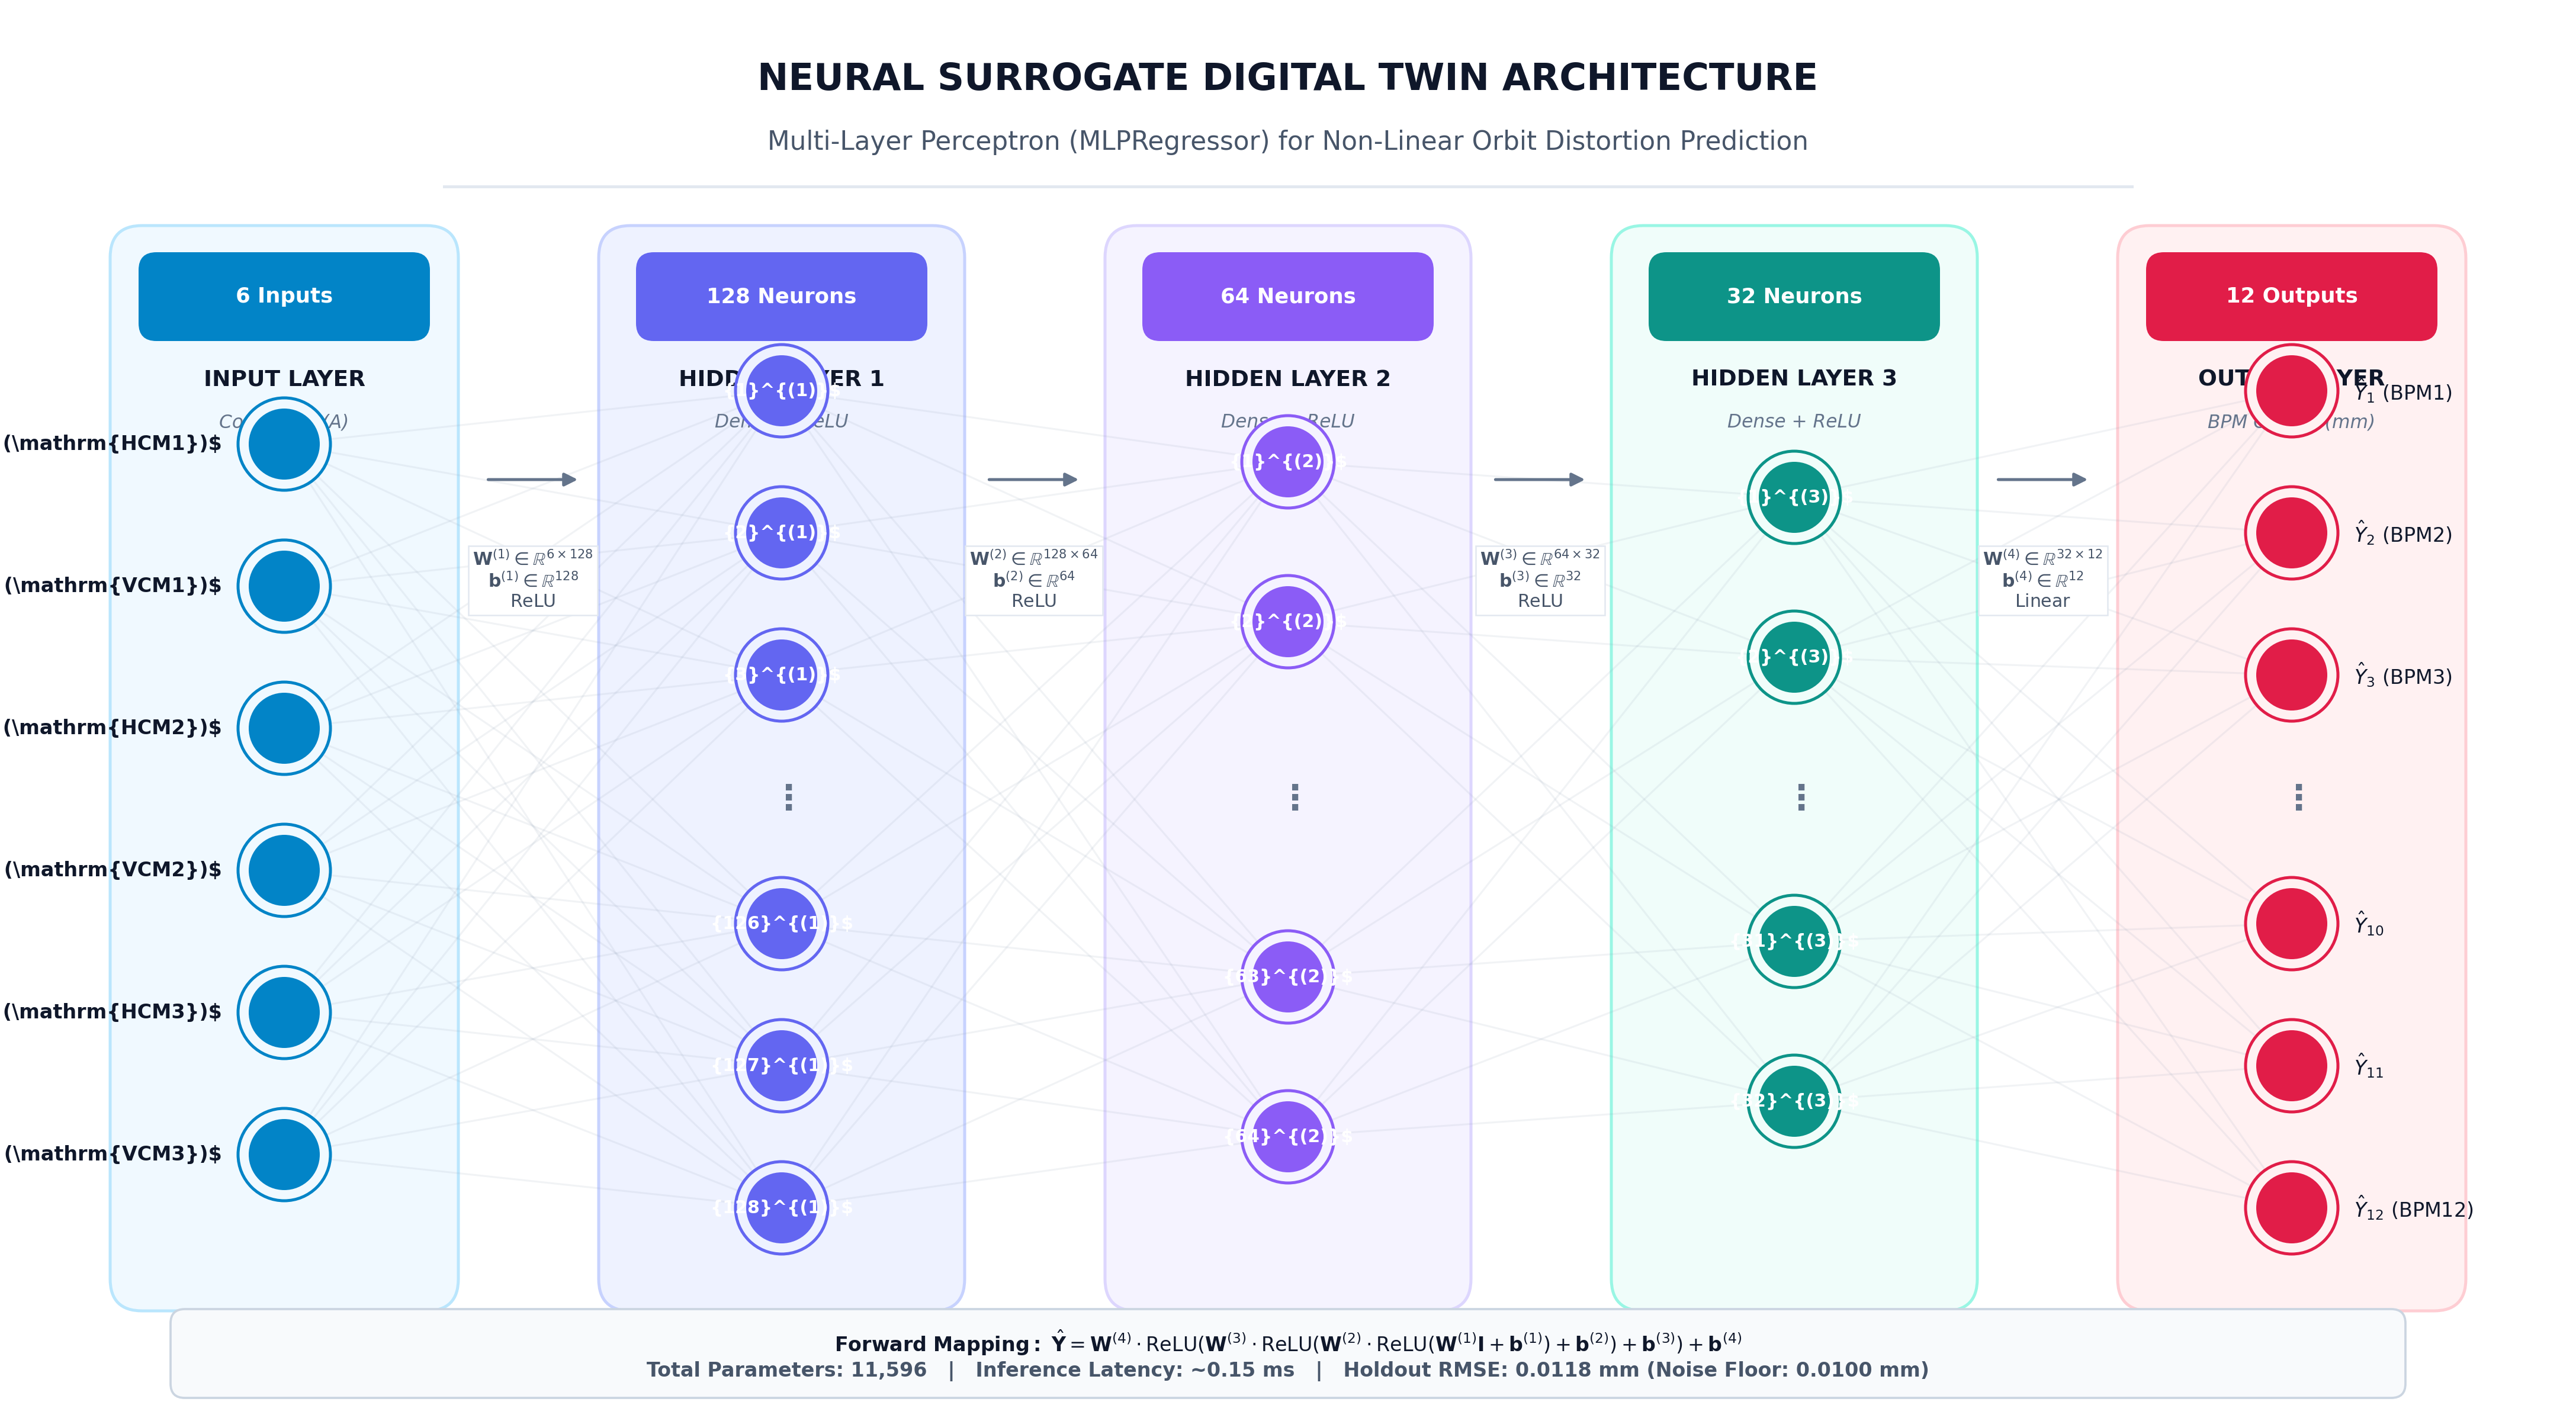
\includegraphics[width=0.90\textwidth]{mlp_schematic.png}
\caption{Architecture of the Multi-Layer Perceptron (MLP) neural surrogate digital twin, mapping 6 dipole corrector currents to 12 BPM transverse orbit offsets through three hidden layers (128, 64, 32 units) with ReLU activations.}
\label{fig:mlp_schematic}
\end{figure}

\begin{itemize}
    \item \textbf{Input Layer ($\mathbb{R}^6$):} Ingests physical magnet actuator setpoints (the 6 corrector currents $I_1, \dots, I_6$).
    \item \textbf{Hidden Layers ($\mathbb{R}^{128} \rightarrow \mathbb{R}^{64} \rightarrow \mathbb{R}^{32}$):} Progressive hierarchical feature representations. Each layer computes:
    \begin{equation}
        \mathbf{h}^{(l)} = \text{ReLU}\left( \mathbf{W}^{(l)} \mathbf{h}^{(l-1)} + \mathbf{b}^{(l)} \right)
    \end{equation}
    \item \textbf{Output Layer ($\mathbb{R}^{12}$):} Linear projection predicting the 12 Beam Position Monitor readings ($\hat{Y}_1, \dots, \hat{Y}_{12}$).
\end{itemize}

\subsection{Loss Functions, Loss Rates \& Metrics: MSE vs.\ RMSE}
Network parameters are trained by minimizing an objective loss function:
\begin{enumerate}
    \item \textbf{Mean Squared Error (MSE) Loss:}
    \begin{equation}
        \mathcal{L}_{\text{MSE}}(\boldsymbol{\theta}) = \frac{1}{N \cdot M} \sum_{i=1}^N \sum_{j=1}^M \left( Y_{i,j} - \hat{Y}_{i,j}(\boldsymbol{\theta}) \right)^2
    \end{equation}
    Smoothly differentiable, penalizing large orbit outliers quadratically.
    
    \item \textbf{Root Mean Squared Error (RMSE) Evaluation Metric:}
    \begin{equation}
        \text{RMSE} = \sqrt{\mathcal{L}_{\text{MSE}}} = \sqrt{\frac{1}{N \cdot M} \sum_{i=1}^N \sum_{j=1}^M \left( Y_{i,j} - \hat{Y}_{i,j} \right)^2}
    \end{equation}
    \textbf{Why RMSE is the preferred metric in beam physics:} It preserves the original physical measurement units (\textbf{millimeters}) and directly reflects accelerator beam orbit distortion standards.
\end{enumerate}

\subsection{Optimization Algorithms: From Gradient Descent to Adam and L-BFGS-B}
During backpropagation, loss gradients $\nabla_{\boldsymbol{\theta}} \mathcal{L}$ are propagated backward to update weights:
\begin{enumerate}
    \item \textbf{Stochastic Gradient Descent (SGD):} $\boldsymbol{\theta}_{t+1} = \boldsymbol{\theta}_t - \eta \nabla_{\boldsymbol{\theta}} \mathcal{L}$, where $\eta$ is the learning rate.
    \item \textbf{Momentum SGD:} $\mathbf{v}_t = \gamma \mathbf{v}_{t-1} + \eta \mathbf{g}_t, \ \boldsymbol{\theta}_{t+1} = \boldsymbol{\theta}_t - \mathbf{v}_t$. Suppresses oscillations in high-curvature ravines.
    \item \textbf{AdaGrad \& RMSprop:} Adapts parameter learning rates based on historical squared gradient accumulation.
    \item \textbf{The Adam Optimizer (Adaptive Moment Estimation):} Combines Momentum (first moment $\mathbf{m}_t$) and RMSprop (second moment $\mathbf{v}_t$):
    \begin{equation}
        \mathbf{m}_t = \beta_1 \mathbf{m}_{t-1} + (1-\beta_1) \mathbf{g}_t, \quad \mathbf{v}_t = \beta_2 \mathbf{v}_{t-1} + (1-\beta_2) \mathbf{g}_t^2
    \end{equation}
    \begin{equation}
        \hat{\mathbf{m}}_t = \frac{\mathbf{m}_t}{1-\beta_1^t}, \quad \hat{\mathbf{v}}_t = \frac{\mathbf{v}_t}{1-\beta_2^t} \implies \boldsymbol{\theta}_{t+1} = \boldsymbol{\theta}_t - \frac{\eta}{\sqrt{\hat{\mathbf{v}}_t} + \epsilon} \hat{\mathbf{m}}_t
    \end{equation}
    Adam scales each parameter's step by its own gradient history, so it needs little tuning and works with mini-batches on large datasets. For this challenge, however, the default Adam run stops after about 85 epochs at a test RMSE of $0.109\text{ mm}$, while a full-batch quasi-Newton solver (\texttt{solver='lbfgs'}) with \texttt{tanh} activations reaches $0.012\text{ mm}$ on the same 1,200 shots.
    \item \textbf{L-BFGS-B (Quasi-Newton with Box Constraints):} Approximates the inverse Hessian $\mathbf{H}^{-1}$ from gradient history. Used for bounded parameter inversion in Baseline~1 and Track~3.
\end{enumerate}

\subsection{Specialized Neural Architectures in Accelerators: Beyond Plain MLPs}
While standard Multi-Layer Perceptrons (MLPs) serve as effective general-purpose regression digital twins for low-dimensional static mappings, accelerator physics and diagnostics frequently present challenges that violate the core assumptions of plain feedforward networks:
\begin{enumerate}
    \item Physical conservation laws (symplectic phase-space area preservation, energy conservation, Maxwell's divergence constraints) are not inherently respected by standard MLPs, leading to unphysical long-term trajectory drift in data-sparse operating regimes.
    \item Dynamic accelerator phenomena exhibit non-Markovian memory, temporal eddy current delays, and magnetic iron-core hysteresis that static feedforward mappings cannot represent.
    \item High-dimensional diagnostic distributions (such as 6D particle bunch phase space and 2D beam profile imaging screens) require specialized spatial equivariance, multiscale localization, or probabilistic continuous manifold compression.
\end{enumerate}
To address these domains, accelerator AI practitioners deploy specialized deep learning topologies (Table~\ref{tab:specialized_nn_architectures}).

\subsubsection{Physics-Informed Neural Networks (PINNs)}
Physics-Informed Neural Networks embed known governing ordinary and partial differential equations directly into the network training loss via automatic differentiation (Raissi et al., 2019). Given a physical differential operator $\mathcal{D}$ (such as Hill's equation $x'' + K(s)x = 0$, Poisson's space-charge equation $\nabla^2 \phi = -\rho / \epsilon_0$, or Maxwell's equations), the PINN objective is formulated as:
\begin{equation}
    \mathcal{L}_{\text{PINN}}(\boldsymbol{\theta}) = \mathcal{L}_{\text{data}}(\boldsymbol{\theta}) + \lambda_{\text{phys}} \mathcal{L}_{\text{physics}}(\boldsymbol{\theta}) = \frac{1}{N} \sum_{i=1}^N \left\| \mathbf{y}_i - f_{\boldsymbol{\theta}}(\mathbf{x}_i) \right\|^2 + \frac{\lambda_{\text{phys}}}{M} \sum_{j=1}^M \left\| \mathcal{D}\left[ f_{\boldsymbol{\theta}} \right](\mathbf{x}_j) \right\|^2
\end{equation}
where $M$ denotes collocation evaluation points distributed across the physical domain, and gradients $\partial f_{\boldsymbol{\theta}} / \partial \mathbf{x}$ are computed analytically through network backpropagation (autograd) without finite-difference grid errors.
\begin{itemize}
    \item \textbf{Why Beyond Plain MLP:} Standard MLPs act as purely empirical black-box interpolators, requiring massive datasets and failing unphysically when extrapolating outside the calibration envelope. PINNs enforce physical conservation principles ($\det \mathbf{J} \equiv 1$, energy conservation), regularizing network weights and ensuring valid physical predictions even in data-sparse lattice sections.
    \item \textbf{Accelerator Applications:} Space-charge field solvers, beam envelope tracking through complex transport lines, and continuous trajectory reconstruction across unmonitored drift sections where BPM diagnostics are absent.
\end{itemize}

\subsubsection{Physics-Guided Recurrent Neural Networks (PRNN, RNN \& LSTM)}
Recurrent Neural Networks (RNNs) and Long Short-Term Memory (LSTM) networks process sequential time-series data by maintaining an internal hidden recurrence state vector $\mathbf{h}_t \in \mathbb{R}^d$:
\begin{equation}
    \mathbf{h}_t = \sigma\left( \mathbf{W}_h \mathbf{h}_{t-1} + \mathbf{W}_x \mathbf{x}_t + \mathbf{b}_h \right), \quad \hat{\mathbf{y}}_t = \mathbf{W}_y \mathbf{h}_t + \mathbf{b}_y
\end{equation}
Physics-Guided Recurrent Neural Networks (PRNNs) augment standard RNN cells by embedding inductive physical models (such as magnetic dipole hysteresis loops, thermal dissipation time constants, or RF cavity decay differential equations) directly into the state transition dynamics.
\begin{itemize}
    \item \textbf{Why Beyond Plain MLP:} Feedforward MLPs treat every observation as independent and identically distributed (i.i.d.), unable to account for historical machine state. PRNNs capture non-Markovian memory, temporal eddy current lag, and magnet cycling history.
    \item \textbf{Accelerator Applications:} Magnetic iron-core hysteresis tracking in ramping synchrotrons and cycling steerers, superconducting RF cavity decay and quenching precursor warning systems, and time-series beam jitter forecasting.
\end{itemize}

\subsubsection{Variational Autoencoders (VAEs)}
Variational Autoencoders (VAEs) are directed probabilistic generative models consisting of an encoder $q_{\boldsymbol{\phi}}(\mathbf{z}|\mathbf{x})$ that maps high-dimensional measurements $\mathbf{x} \in \mathbb{R}^D$ into a continuous low-dimensional latent Gaussian distribution $\mathbf{z} \sim \mathcal{N}(\boldsymbol{\mu}_{\mathbf{z}}, \boldsymbol{\Sigma}_{\mathbf{z}})$, and a decoder $p_{\boldsymbol{\theta}}(\mathbf{x}|\mathbf{z})$ that reconstructs the observation (Kingma \& Welling, 2013). VAEs are trained by maximizing the Evidence Lower Bound (ELBO):
\begin{equation}
    \mathcal{L}_{\text{ELBO}}(\boldsymbol{\theta}, \boldsymbol{\phi}) = \mathbb{E}_{q_{\boldsymbol{\phi}}(\mathbf{z}|\mathbf{x})}\left[ \log p_{\boldsymbol{\theta}}(\mathbf{x}|\mathbf{z}) \right] - D_{\text{KL}}\left( q_{\boldsymbol{\phi}}(\mathbf{z}|\mathbf{x}) \,\big\|\, p(\mathbf{z}) \right)
\end{equation}
where the first term is the reconstruction fidelity and the second term is the Kullback-Leibler divergence constraining the latent posterior against a standard Gaussian prior $p(\mathbf{z}) = \mathcal{N}(\mathbf{0}, \mathbf{I})$.
\begin{itemize}
    \item \textbf{Why Beyond Plain MLP:} While MLPs perform discrete deterministic regression, VAEs learn smooth, continuous, probabilistic latent manifolds that enable unsupervised clustering, anomaly scoring, and synthetic generative sampling.
    \item \textbf{Accelerator Applications:} 6D particle bunch phase-space distribution compression, unsupervised anomaly detection (identifying abnormal beam loss spike precursors or impending vacuum trips), and generative synthesis of realistic machine operating states for virtual commissioning.
\end{itemize}

\subsubsection{Convolutional Encoder-Decoders (U-Net \& CNNs)}
Convolutional Neural Networks (CNNs) process multi-dimensional spatial diagnostic arrays by sharing localized filter kernels across the input, preserving translation equivariance: $\text{Conv}(\mathbf{X})_{i,j} = \sum_{u,v} K_{u,v} X_{i-u, j-v}$. The U-Net topology (Ronneberger et al., 2015) extends this into a symmetric encoder-decoder:
\begin{enumerate}
    \item \textbf{Contracting Encoder Path:} Successive convolution and pooling layers downsample spatial resolution while progressively extracting hierarchical feature abstractions.
    \item \textbf{Expanding Decoder Path:} Successive transpose convolutions (or bilinear upsampling) restore original spatial dimensions.
    \item \textbf{Cross-Layer Skip Connections:} Direct tensor concatenation bridges encoder feature maps to matching decoder stages:
    \begin{equation}
        \mathbf{x}_{\text{dec}}^{(l)} = \text{Conv}\left( \text{Upsample}\left(\mathbf{x}_{\text{dec}}^{(l+1)}\right) \;\oplus\; \mathbf{x}_{\text{enc}}^{(l)} \right)
    \end{equation}
    retaining fine, high-resolution edge details that would otherwise be lost in the bottleneck compression.
\end{enumerate}
\begin{itemize}
    \item \textbf{Why Beyond Plain MLP:} A standard MLP applied to a $1024 \times 1024$ diagnostic camera image requires millions of weights per neuron, causing parameter explosion and discarding 2D spatial pixel correlations. U-Net leverages spatial parameter sharing and multiscale skip pathways to achieve pixel-level accuracy.
    \item \textbf{Accelerator Applications:} Real-time transverse beam profile reconstruction from scintillation screen cameras (YAG, OTR), transverse halo segmentation, phase-space tomography, and 2D/3D magnet fringe field map interpolation.
\end{itemize}

\begin{table}[h!]
\centering
\small
\setlength{\tabcolsep}{4pt}
\begin{tabular}{@{}p{2.5cm} p{3.3cm} p{4.2cm} p{4.7cm}@{}}
\toprule
\textbf{Architecture} & \textbf{Core Mechanism} & \textbf{Why Beyond Plain MLP} & \textbf{Key Accelerator Use Cases} \\
\midrule
\textbf{PINN}\newline (Physics-Informed) & ODE/PDE residual in loss: $\mathcal{L}_{\text{data}} + \lambda_{\text{phys}}\|\mathcal{D}[f]\|^2$ via autograd & Enforces physical conservation ($\det\mathbf{J}\equiv 1$, energy) in data-sparse domains & Space-charge Poisson solvers, envelope equations, unmonitored drift prediction \\
\midrule
\textbf{PRNN / RNN}\newline (Physics-Guided Recurrent) & Dynamic recurrent hidden state $\mathbf{h}_t = \sigma(\mathbf{W}_h \mathbf{h}_{t-1} + \dots)$ + physical delay biases & Models non-Markovian memory, temporal eddy current lags, and state dependence & Magnetic hysteresis tracking during cycling, superconducting RF cavity decay, jitter forecasting \\
\midrule
\textbf{VAE}\newline (Variational Autoencoder) & Probabilistic latent space $\mathbf{z}\sim\mathcal{N}(\boldsymbol{\mu},\boldsymbol{\Sigma})$ via ELBO optimization & Unsupervised generative density modeling; continuous manifold representation & 6D particle bunch phase-space compression, unsupervised trip/anomaly detection, virtual diagnostics \\
\midrule
\textbf{U-Net / CNN}\newline (Convolutional Encoder-Decoder) & Multiscale contracting \& expanding paths with cross-layer skip connections & Exploits spatial translation equivariance; retains fine pixel details with global context & Transverse beam profile camera reconstruction (YAG/OTR), halo segmentation, 3D field map interpolation \\
\bottomrule
\end{tabular}
\caption{Specialized deep neural network architectures deployed in modern particle accelerator physics and beamline diagnostics.}
\label{tab:specialized_nn_architectures}
\end{table}

\subsection{Dataset Partitioning \& The Bias-Variance Tradeoff}
To prevent memorization of diagnostic noise, data is partitioned into:
\begin{itemize}
    \item \textbf{Training Set (80\%, 1,200 shots):} Used directly for loss gradient computation and parameter updates.
    \item \textbf{Validation Set (Optional):} Monitored across epochs for early stopping before overfitting occurs.
    \item \textbf{Test / Holdout Set (20\%, 300 shots):} Strictly isolated during training to provide an unbiased benchmark on unseen accelerator states.
\end{itemize}
\begin{itemize}
    \item \textbf{Underfitting (High Bias):} Linear models cannot capture the cubic magnetic core saturation.
    \item \textbf{Overfitting (High Variance):} Over-parameterized models memorizing Gaussian sensor noise ($\sigma = 10\ \mu\text{m}$). Prevented using $L_2$ weight regularization (`alpha=1e-4`).
\end{itemize}

\subsection{Challenge Implementation \& Empirical Benchmark}
In Step 3 of the challenge notebook, $1,500$ experimental samples are synthesized uniformly across current boundaries $[-3.0\text{ A}, +3.0\text{ A}]$:
\begin{lstlisting}[language=Python]
n_train_samples = 1500
X_offline = np.random.uniform(-3.0, 3.0, size=(n_train_samples, env.n_correctors))
Y_linear = X_offline @ env.R
Y_sat = - 0.015 * (X_offline**3) @ env.R
bpm_noise = np.random.normal(0, 0.010, size=(n_train_samples, env.n_bpms))
Y_offline = Y_linear + Y_sat + bpm_noise

X_train, X_test, Y_train, Y_test = train_test_split(
    X_offline, Y_offline, test_size=0.20, random_state=42
)

# Train Linear Ridge vs Deep MLP Regressor
linear_model = Ridge(alpha=1.0).fit(X_train, Y_train)
surrogate_model = MLPRegressor(
    hidden_layer_sizes=(128, 64, 32), activation='relu',
    solver='adam', alpha=1e-4, max_iter=400, random_state=42
).fit(X_train, Y_train)
\end{lstlisting}

\begin{table}[h!]
\centering
\resizebox{\textwidth}{!}{%
\begin{tabular}{@{}lcccp{6.5cm}@{}}
\toprule
\textbf{Model} & \textbf{Parameters} & \textbf{Holdout RMSE} & \textbf{Inference Latency} & \textbf{What it captures} \\
\midrule
Linear Ridge ($\lambda=1.0$) & 84 & $0.082\text{ mm}$ & $< 0.01\text{ ms}$ & Linear optics only; misses saturation. \\
Reference MLP (ReLU, Adam, 128-64-32) & 11,628 & $0.109\text{ mm}$ & $\approx 0.1\text{ ms}$ & Under-trained: Adam stops after about 85 epochs, and the result is worse than the linear model. \\
Tuned MLP (\texttt{tanh}, \texttt{lbfgs}, 64-64) & 5,388 & $\mathbf{0.012\text{ mm}}$ & $\approx 0.1\text{ ms}$ & Linear response and cubic saturation, down to the sensor noise. \\
\bottomrule
\end{tabular}%
}
\caption{Holdout validation on the 300 test shots of the notebook dataset (1,500 shots over $\pm 3.0\text{ A}$, \texttt{random\_state=42}).}
\label{tab:surrogate_perf}
\end{table}

\begin{infobox}[Insight: Judge a Surrogate by its Holdout Error]
A larger network is not automatically a better surrogate. The reference MLP has 140 times more parameters than the linear model and still predicts worse, because its training stops early. The tuned MLP has half as many parameters as the reference and reaches $0.012\text{ mm}$, close to the $0.010\text{ mm}$ limit set by the sensor noise; no model can do better on noisy test data. Improving the surrogate is \texttt{TODO 1}.
\end{infobox}


\section{Closed-Loop Control Paradigms}

\subsection{Closed-Loop Control Architecture \& Feedback Loop}
In particle accelerators, closed-loop orbit correction iteratively stabilizes the beam position against external ground vibrations, power-supply ripple, and thermal drifts. At each discrete iteration step $t \in [0, 50]$, the closed-loop orbit correction system operates over transverse beam position monitor measurements and steerer magnet currents:
\begin{enumerate}
    \item \textbf{Diagnostic Observation:} The Beam Position Monitors (BPMs) record the current orbit distortion vector $\mathbf{Y}_t \in \mathbb{R}^{12}$ (in millimeters), which includes unperturbed trajectory, corrector deflections, non-linear saturation, and Gaussian sensor noise $\boldsymbol{\epsilon} \sim \mathcal{N}(\mathbf{0}, \sigma^2 \mathbf{I})$ with $\sigma = 0.010\text{ mm}$.
    \item \textbf{Controller Policy Calculation:} The controller receives the observation $\mathbf{Y}_t$ (and optional runtime metadata such as current steerer magnet settings $\mathbf{I}_t$) and computes an incremental adjustment action $\Delta\mathbf{I}_t \in [-0.8, +0.8]^6\text{ A}$.
    \item \textbf{Actuator Execution \& State Update:} The dipole correctors update their total current settings:
    \begin{equation}
        \mathbf{I}_{t+1} = \text{clip}\left(\mathbf{I}_t + \Delta\mathbf{I}_t, \ -5.0, \ +5.0\right)\text{ A}
    \end{equation}
    \item \textbf{Convergence Evaluation:} The updated beam trajectory $\mathbf{Y}_{t+1}$ is measured. The correction terminates successfully if the transverse root-mean-square orbit distortion satisfies:
    \begin{equation}
        \text{RMS}_{t+1} = \sqrt{\frac{1}{12}\sum_{j=1}^{12} Y_{t+1, j}^2} < 0.030\text{ mm}
    \end{equation}
    If the threshold is not reached within $t = 50$ steps, the episode truncates as a failure.
\end{enumerate}

To solve this closed-loop alignment task, the benchmark evaluates three distinct learning paradigms alongside the classical analytical baseline:
\begin{itemize}
    \item \textbf{Baseline 0 (Classical SVD):} Directly inverts the linear Orbit Response Matrix (ORM) using the Moore-Penrose pseudo-inverse.
    \item \textbf{Track 1 (Supervised Neural Inversion):} Learns an offline forward digital twin $f_{\boldsymbol{\theta}}(\mathbf{I})$ from calibration data and numerically inverts it via bounded optimization at each step.
    \item \textbf{Track 2 (Reinforcement Learning Policy):} Learns an end-to-end feedback policy mapping measured orbit errors directly to corrective kicks, leveraging a physics prior with learned residuals and adaptive damping.
    \item \textbf{Track 3 (Bayesian Optimization):} Employs a Gaussian Process surrogate to quantify predictive uncertainty and balances exploration versus exploitation via Lower Confidence Bound (LCB) minimization.
\end{itemize}

\subsection{Baseline 0: Classical SVD Pseudo-Inverse Controller}
In standard accelerator control rooms, Singular Value Decomposition (SVD) of the transpose response matrix $\mathbf{R}^T = \mathbf{U} \boldsymbol{\Sigma} \mathbf{V}^T$ provides the Moore-Penrose pseudo-inverse:
\begin{equation}
    (\mathbf{R}^T)^\dagger = \mathbf{V} \boldsymbol{\Sigma}^{-1} \mathbf{U}^T
\end{equation}
The closed-loop correction action per step is:
\begin{equation}
    \Delta \mathbf{I} = \text{clip}\left( - \alpha \cdot (\mathbf{R}^T)^\dagger \cdot \mathbf{Y}_{\text{obs}}, \ -0.8, \ +0.8 \right)
\end{equation}
where $\alpha \approx 0.45$ is the feedback gain.
While computationally instantaneous, SVD assumes linearity. Gains up to about $1.2$ converge fastest (about 3.7 steps at $\alpha = 1.2$ versus 9.4 at $0.45$); above that the controller overshoots.

\subsection{Baseline 1 (Track 1): Model-Based Optimization via Digital Twin Inversion}
Rather than inverting an analytical matrix, Baseline 1 optimizes corrective kicks directly through the forward neural surrogate $f_{\boldsymbol{\theta}}(\mathbf{I})$, which maps the total corrector current to the orbit, using SciPy's \texttt{L-BFGS-B} algorithm (the kick found within $\pm 5\text{ A}$ is then clipped to the $\pm 0.8\text{ A}$ step limit):
\begin{equation}
    \min_{\Delta \mathbf{I}} \mathcal{L}(\Delta \mathbf{I}) = \left\| \mathbf{Y}_{\text{obs}} - f_{\boldsymbol{\theta}}(\mathbf{I}) + f_{\boldsymbol{\theta}}(\mathbf{I} + \Delta \mathbf{I}) \right\|_2^2 + \lambda \|\Delta \mathbf{I}\|_2^2 \quad \text{s.t.} \quad \Delta \mathbf{I} \in [-5.0\text{ A}, +5.0\text{ A}]^6
\end{equation}

\begin{lstlisting}[language=Python]
class SupervisedMLPController:
    def __init__(self, surrogate):
        self.surrogate = surrogate

    def act(self, obs, info=None):
        I_now = np.asarray(info["currents"]) if info else np.zeros(6)   # present total current
        f_now = self.surrogate.predict(I_now.reshape(1, -1))[0]
        def objective(delta_I):
            pred = self.surrogate.predict((I_now + delta_I).reshape(1, -1))[0]
            residual = obs - f_now + pred                                  # predicted next orbit
            return np.sum(residual**2) + 0.0001 * np.sum(delta_I**2)
            
        res = opt.minimize(objective, np.zeros(6), bounds=[(-5.0, 5.0)]*6, method='L-BFGS-B')
        return np.clip(res.x, -0.8, 0.8)
\end{lstlisting}
When the surrogate accurately anticipates non-linear saturation falloff, Baseline 1 converges in about 4 iterations (4 steps on test seed 42, against 9 for classical SVD). Here $\mathbf{I}$ is the present total corrector current from \texttt{info["currents"]}, so the objective uses the predicted next orbit at every step. With the reference MLP settings (test RMSE about $0.11\text{ mm}$) it succeeds on all 30 seeds and scores 779.169, because the feedback loop corrects much of the model error: every step starts from a fresh measurement. A more accurate surrogate (a small \texttt{tanh} network trained with \texttt{lbfgs}, test RMSE about $0.012\text{ mm}$) lands closer to the noise floor: 902.5 with the same controller, and 924.2 with the worked-solution controller.

\subsubsection{Supervised Learning Hyperparameter Taxonomy}
Table~\ref{tab:sl_hyperparams} outlines the primary hyperparameters governing surrogate training.

\begin{table}[h!]
\centering
\small
\begin{tabular}{@{}p{3.2cm} p{2.6cm} p{9.2cm}@{}}
\toprule
\textbf{Hyperparameter} & \textbf{Typical Value} & \textbf{Physical Meaning \& Role in Accelerator Surrogate} \\
\midrule
\textbf{\color{tunablered}Learning Rate ($\eta$)$^*$} & $10^{-3}$ (Adam) & Step size along gradient. Too large diverges; too small stagnates in flat loss ravines. \\
\textbf{\color{tunablered}Batch Size ($B$)$^*$} & $32 - 128$ & Samples per gradient step. Mini-batching provides regularization against sensor jitter. \\
\textbf{\color{tunablered}Layer Architecture$^*$} & $(128, 64, 32)$ & Hidden depth and width. Sufficient capacity to represent cubic saturation without memorizing noise. \\
\textbf{\color{tunablered}Activation Function ($\sigma$)$^*$} & \texttt{relu} (default), \texttt{tanh} & Non-linearity in hidden layers (\texttt{MLPRegressor} offers \texttt{relu}, \texttt{tanh}, \texttt{logistic}, \texttt{identity}). The output layer is always linear. \\
\textbf{\color{tunablered}Solver$^*$} & \texttt{adam} (default), \texttt{lbfgs} & Training algorithm. \texttt{lbfgs} is full-batch and suits small, smooth datasets like this one. \\
\textbf{\color{tunablered}$L_2$ Regularization ($\alpha$)$^*$} & $10^{-4}$ & Weight decay penalty $\frac{1}{2}\alpha\|\mathbf{W}\|_2^2$ suppressing overfitting to diagnostic noise ($\sigma = 10\ \mu\text{m}$). \\
\textbf{\color{tunablered}Max Epochs / Early Stop$^*$} & 400 epochs, tol=$10^{-4}$ & Training stops when the loss improves by less than \texttt{tol} for 10 epochs (after about 85 epochs with the defaults), or at \texttt{max\_iter}. \\
\bottomrule
\end{tabular}
\caption{Hyperparameter taxonomy for supervised neural surrogate modeling (\textbf{\color{tunablered}$^*$Highlighted in red: Tunable by participants in notebook TODO 1}).}
\label{tab:sl_hyperparams}
\end{table}

\subsection{Track 2: Closed-Loop RL Policy with Physics Prior and Adaptive Damping}
Model-based iterative optimization takes about $27\text{ ms}$ per step for Baseline~1. In contrast, a direct closed-loop policy executes in well under $0.1\text{ ms}$~\cite{kain2020sample}.
High-performing accelerator policy agents integrate an analytical \textbf{physics prior} with a learned parameter residual and dynamic step damping:
\begin{equation}
    \Delta \mathbf{I}(t) = \gamma(t) \cdot \left[ \underbrace{- \alpha (\mathbf{R}^T)^\dagger \mathbf{Y}}_{\text{Analytical Physics Prior}} + \underbrace{\mathbf{W}_{\text{learned}}\mathbf{Y} + \mathbf{b}}_{\text{Learned Residual Offset}} \right]
\end{equation}
\begin{equation}
    \gamma(t) = \frac{1.0}{1.0 + 0.03 \cdot t}
\end{equation}
The damping factor $\gamma(t)$ reduces the kick authority as the episode proceeds ($0.77$ at $t = 10$, $0.53$ at $t = 30$), so that late kicks respond less to the $10\ \mu\text{m}$ sensor noise near the $0.030\text{ mm}$ boundary. In the reference agent, $\mathbf{W}_{\text{learned}}$ and $\mathbf{b}$ start at zero and are not trained, so it behaves as a damped pseudo-inverse controller (590.559 points). It scores below Baseline~0 (635.277) because, at the low gain of 0.45, the damping only slows it down. Training or tuning the residual, raising the gain, or replacing the prior with a saturation-aware model inversion is the Track~2 task.

\paragraph{Damping is a trade-off, not a free gain.} Table~\ref{tab:damping} gives the score of the plain pseudo-inverse on the 30 seeds. At low gain, damping only costs steps. At gain 1.0 a little damping improves the landing precision enough to pay for the extra step; at gain 1.2 it does not. In the benchmark an episode ends at the first reading below $0.030\text{ mm}$, so damping matters less here than in continuous feedback, where the orbit must be held near the noise floor indefinitely.

\begin{table}[h!]
\centering
\small
\begin{tabular}{@{}cccc@{}}
\toprule
\textbf{Gain $\alpha$} & \textbf{No damping} & \textbf{$\kappa = 0.03$} & \textbf{$\kappa = 0.1$} \\
\midrule
0.45 & 635.3 (9.4 steps) & 590.6 (10.8 steps) & 503.8 (15.9 steps) \\
1.0 & 765.3 (4.3 steps) & \textbf{782.8} (4.7 steps) & 721.1 (5.3 steps) \\
1.2 & \textbf{822.1} (3.7 steps) & 808.9 (4.0 steps) & 746.4 (4.4 steps) \\
\bottomrule
\end{tabular}
\caption{Benchmark score (mean steps) of the plain pseudo-inverse controller with damping $\gamma(t) = 1/(1 + \kappa t)$.}
\label{tab:damping}
\end{table}

\subsubsection{Reinforcement Learning MDP Hyperparameter Taxonomy}
Table~\ref{tab:rl_hyperparams} outlines the primary hyperparameters in the closed-loop MDP orbit alignment formulation.

\begin{table}[h!]
\centering
\small
\begin{tabular}{@{}p{3.2cm} p{2.6cm} p{9.2cm}@{}}
\toprule
\textbf{Hyperparameter} & \textbf{Typical Value} & \textbf{Physical Meaning \& Role in Orbit Control} \\
\midrule
\textbf{\color{tunablered}Discount Factor ($\gamma$)$^*$} & $0.95 - 0.99$ & Temporal horizon weight. High $\gamma$ prioritizes terminal alignment ($< 0.030\text{ mm}$) over step cost. \\
\textbf{\color{tunablered}Policy LR ($\eta_\pi$)$^*$} & $10^{-4} - 10^{-3}$ & Step size for policy parameter updates. Must remain small to avoid policy collapse under sensor noise. \\
\textbf{\color{tunablered}Exploration Noise ($\sigma$)$^*$} & $\mathcal{N}(0, 0.05^2)\text{ A}$ & Action perturbations during training to probe saturation limits without damaging hardware. \\
\textbf{\color{tunablered}Harmonic Damping ($\kappa$)$^*$} & $\approx 0.03$ & Authority schedule $\gamma(t) = 1/(1+\kappa t)$ reducing late kick authority; a trade-off between steps and landing precision. \\
\textbf{\color{tunablered}Feedback Gain ($\alpha$)$^*$} & $0.45 \to 1.2$ & Feedback scaling factor; higher gains converge faster, and above about 1.2 the controller overshoots. \\
\textbf{\color{tunablered}Reward Weights ($w_{\text{rms}}, w_{\text{act}}$)$^*$} & $w_{\text{rms}}=10, w_{\text{act}}=0.01$ & Balances orbit minimization priority against coil resistive heating and power supply strain. \\
\textbf{\color{tunablered}Step Penalty ($c_{\text{step}}$)$^*$} & $0.5\text{ pts/step}$ & Time penalty encouraging minimum-step convergence to maximize benchmark speed score (up to 300 pts). \\
\textbf{\color{tunablered}Success Bonus ($b_{\text{term}}$)$^*$} & $50.0\text{ pts}$ & Large positive terminal reward upon reaching $\text{RMS} < 0.030\text{ mm}$. \\
\bottomrule
\end{tabular}
\caption{Hyperparameter taxonomy for closed-loop reinforcement learning orbit control (\textbf{\color{tunablered}$^*$Highlighted in red: Tunable by participants in notebook TODO 2}). The discount factor, policy learning rate and exploration noise apply only if you add your own RL training loop: the reference agent has no training step.}
\label{tab:rl_hyperparams}
\end{table}

\subsection{Track 3: Closed-Loop Bayesian Optimization with Gaussian Processes}
Bayesian Optimization (BO) provides sample-efficient optimization in high-dimensional non-linear systems by combining a probabilistic surrogate model with an acquisition function~\cite{roussel2023turnkey, edelen2020machine}. In our closed-loop architecture, a Gaussian Process (GP) regressor models the mapping from the total corrector currents $\mathbf{I}$ to the orbit response:
\begin{equation}
    \hat{\mathbf{Y}}(\mathbf{I}) \sim \mathcal{GP}\left(\mathbf{m}(\mathbf{I}), \mathbf{K}(\mathbf{I}, \mathbf{I}')\right)
\end{equation}
where $\mathbf{m}(\cdot)$ is the prior mean function and $\mathbf{K}(\cdot, \cdot)$ is a covariance kernel. To capture the smooth physics of magnetic core saturation while accounting for BPM diagnostic noise ($\sigma = 0.010\text{ mm}$), we employ a Mat\'ern-5/2 kernel augmented with a white noise kernel:
\begin{equation}
    k(\mathbf{x}, \mathbf{x}') = \sigma_f^2 \left( 1 + \sqrt{5}\frac{r}{\ell} + \frac{5}{3}\frac{r^2}{\ell^2} \right) \exp\left( -\sqrt{5}\frac{r}{\ell} \right) + \sigma_n^2 \delta(\mathbf{x}, \mathbf{x}')
\end{equation}
where $r = \|\mathbf{x} - \mathbf{x}'\|_2$, $\ell$ is the characteristic length scale, and $\sigma_n = 0.010\text{ mm}$.

\subsubsection{Epistemic Uncertainty \& Acquisition Function}
Unlike standard point-prediction neural networks, the Gaussian Process yields both a posterior mean $\boldsymbol{\mu}(\mathbf{I})$ and a posterior standard deviation $\boldsymbol{\sigma}(\mathbf{I})$ quantifying epistemic uncertainty.
We evaluate candidate corrective kicks using the Lower Confidence Bound (LCB) acquisition function:
\begin{equation}
    \alpha_{\text{LCB}}(\Delta \mathbf{I}) = \text{RMS}\left( \mathbf{Y}_{\text{obs}} - \boldsymbol{\mu}(\mathbf{I}) + \boldsymbol{\mu}(\mathbf{I} + \Delta \mathbf{I}) \right) - \kappa \cdot \overline{\boldsymbol{\sigma}}(\mathbf{I} + \Delta \mathbf{I}) + \lambda \|\Delta \mathbf{I}\|_2^2
\end{equation}
where $\mathbf{I}$ is the present total current, $\overline{\boldsymbol{\sigma}}$ is the posterior standard deviation averaged over the 12 BPMs, and $\kappa \ge 0$ balances exploitation (minimizing predicted orbit RMS) with exploration (reducing uncertainty in non-linear saturation regimes). When $\kappa = 0$, the controller performs pure exploitation of the posterior mean (holdout RMSE $0.028\text{ mm}$ from 300 shots, four times more accurate than the reference MLP trained on 1,200), converging in about \textbf{3.6 steps} on average across the benchmark suite (878.384 points).

\paragraph{Closed-loop control, offline model.} The controller is closed-loop: at every step it re-solves the acquisition problem from the latest BPM reading $\mathbf{Y}_{\text{obs}}$. Its model, however, is not updated online. The reference GP is fitted once on about 300 calibration shots and stays fixed for the whole benchmark, which makes it structurally close to Track~1 (an offline surrogate inverted at every step) with uncertainty available through $\kappa$. Classic Bayesian optimization adds each new (kick, observed orbit) pair to the GP and refits it; participants can do this from a \texttt{step\_callback} registered in the notebook's \texttt{CALLBACKS}, turning Track~3 into true online Bayesian optimization.

\begin{lstlisting}[language=Python]
class BayesianOptimizationController:
    def __init__(self, gp_surrogate, kappa=0.0, l2_reg=0.0001):
        self.gp = gp_surrogate
        self.kappa = kappa
        self.l2_reg = l2_reg

    def act(self, obs, info=None):
        I_now = np.asarray(info["currents"]) if info else np.zeros(6)   # present total current
        mu_now = self.gp.predict(I_now.reshape(1, -1))[0]
        def acquisition_lcb(delta_I):
            pred_mean, pred_std = self.gp.predict((I_now + delta_I).reshape(1, -1), return_std=True)
            res = obs - mu_now + pred_mean[0]                              # predicted next orbit
            rms_pred = np.sqrt(np.mean(res**2))
            unc = np.mean(pred_std)
            return float(rms_pred - self.kappa * unc + self.l2_reg * np.sum(delta_I**2))

        res = opt.minimize(acquisition_lcb, np.zeros(6), bounds=[(-5.0, 5.0)]*6, method='L-BFGS-B')
        return np.clip(res.x, -0.8, 0.8)
\end{lstlisting}

\subsubsection{Bayesian Optimization \& Gaussian Process Hyperparameter Taxonomy}
Table~\ref{tab:bo_hyperparams} summarizes the key hyperparameters defining the Gaussian Process surrogate and acquisition policy.

\begin{table}[h!]
\centering
\small
\begin{tabular}{@{}p{3.2cm} p{2.6cm} p{9.2cm}@{}}
\toprule
\textbf{Hyperparameter} & \textbf{Typical Value} & \textbf{Role in Gaussian Process \& Beam Alignment} \\
\midrule
\textbf{\color{tunablered}Kernel Function ($k$)$^*$} & Mat\'ern-5/2 & Twice-differentiable covariance modeling physical saturation without excessive RBF stiffness. \\
\textbf{\color{tunablered}Lengthscales ($\ell_k$)$^*$} & $\ell \sim 1.0 - 2.5\text{ A}$ & Input correlation distance per magnet actuator. Sets how rapidly orbit effects decorrelate in current space. \\
\textbf{\color{tunablered}Signal Variance ($\sigma_f^2$)$^*$} & $\sigma_f \sim 1.5\text{ mm}$ & Expected vertical amplitude variation of transverse orbit distortions across the operating domain. \\
\textbf{Noise Variance Floor ($\sigma_n^2$)} & $\sigma_n = 0.010\text{ mm}$ & \textbf{Fixed} physical sensor noise floor ($10\ \mu\text{m}$); \emph{do not modify}. Prevents GP overfitting. \\
\textbf{\color{tunablered}Exploration Weight ($\kappa$)$^*$} & $\kappa = 0.0 \to 1.5$ & Trade-off parameter in LCB. $\kappa > 0$ probes unmapped saturation; $\kappa = 0$ exploits calibrated mean. \\
\textbf{\color{tunablered}Action Penalty ($\lambda$)$^*$} & $10^{-4}$ & Regularizes delta kick effort to avoid unnecessary high-current excursions. \\
\textbf{\color{tunablered}Model Updating$^*$} & Offline / Online Refit & Fixed 300-shot calibration GP (offline baseline) or online recursive GP updating from \texttt{step\_callback}. \\
\bottomrule
\end{tabular}
\caption{Hyperparameter taxonomy for Bayesian optimization with Gaussian process surrogates (\textbf{\color{tunablered}$^*$Highlighted in red: Tunable by participants in notebook TODO 3}).}
\label{tab:bo_hyperparams}
\end{table}


\section{Mini-Hackathon Problem Formulation \& Gymnasium Contract}

\subsection{Gymnasium Environment Specification (\texttt{AcceleratorOrbitGymEnv})}
The benchmark simulation models the 15-meter transport line wrapped inside a standard Farama Gymnasium environment interface:
\begin{itemize}
    \item \textbf{Observation Space:} $\text{Box}(-10.0, +10.0, \text{shape}=(12,), \text{dtype}=\text{float32})$ (Transverse BPM readings in mm).
    \item \textbf{Action Space:} $\text{Box}(-0.8, +0.8, \text{shape}=(6,), \text{dtype}=\text{float32})$ (Per-step delta currents $\Delta \mathbf{I}$ in Amperes).
    \item \textbf{State Dynamics:} Cumulative magnet current $\mathbf{I}_{t+1} = \text{clip}(\mathbf{I}_t + \Delta \mathbf{I}_t, -5.0, +5.0)\text{ A}$, accounting for non-linear core saturation $-0.015 \cdot \mathbf{I}^3 \cdot \mathbf{R}$ and Gaussian diagnostic jitter $\sigma = 0.010\text{ mm}$.
    \item \textbf{Termination Criteria:} Triggered when $\text{RMS} < 0.030\text{ mm}$ (success); truncated if step count reaches $50$ (failure).
    \item \textbf{Step Reward:}
    \begin{equation}
        r_t = - 10 \cdot \text{RMS}_{t+1} - 0.01 \cdot \|\Delta \mathbf{I}_t\|_2^2 - c_{\text{step}} + (50.0 \text{ if } \text{RMS}_{t+1} < 0.030\text{ mm} \text{ else } 0.0)
    \end{equation}
\end{itemize}

\subsection{The Three Parallel Challenge Tracks}
Participants solve the beam alignment challenge by competing in one or more parallel algorithmic tracks within \texttt{Single\_Notebook\_Beam\_Orbit\_Predictor\_Participant.ipynb}:
\begin{enumerate}
    \item \textbf{Track 1 (Supervised Digital Twin Inversion, \texttt{TODO 1}):}
    Train a non-linear Multi-Layer Perceptron ($f_{\boldsymbol{\theta}}$) on offline tracking data to model the cubic iron core saturation. In operations, solve a bounded optimization problem per step via SciPy \texttt{L-BFGS-B} to invert the digital twin.
    
    \item \textbf{Track 2 (Closed-Loop Reinforcement Learning Policy, \texttt{TODO 2}):}
    Design a fast closed-loop policy that combines an analytical pseudo-inverse physics prior with a learned or tuned residual and step damping $\gamma(t) = 1.0 / (1.0 + \kappa \cdot t)$. If you train a policy with RL, the environment's reward weights let you favor fast convergence.
    
    \item \textbf{Track 3 (Bayesian Optimization Controller, \texttt{TODO 3}):}
    Fit a Gaussian Process surrogate with Mat\'ern-5/2 kernel and diagnostic noise floor. Optimize a Lower Confidence Bound (LCB) acquisition function to balance epistemic uncertainty exploration against exploitation of predicted orbit corrections under non-linear saturation.
\end{enumerate}

\subsection{Standardized 30-Seed Evaluation \& Multi-Objective Scoring Formula}
To eliminate evaluation bias, all competitor policies are evaluated across \textbf{30 standardized evaluation seeds} (\texttt{range(1, 31)}).
Each seed is scored from $0$ to $1000$ points and the official challenge score is the mean:
\begin{equation}
    \text{Score} = \frac{1}{30}\sum_{k=1}^{30} s_k
\end{equation}
where the per-seed score $s_k \in [0, 1000]$ is evaluated as:
\begin{equation}
    s_k = \begin{cases}
    400 + 300\,\max\!\left(0,\,\dfrac{20 - n_k}{19}\right) + 300\,\mathrm{clip}\!\left(\dfrac{\ln(0.030/\text{RMS}_k)}{\ln(0.030/0.010)},\,0,\,1\right) & \text{if seed } k \text{ succeeds} \\
    0 & \text{otherwise}
    \end{cases}
\end{equation}

\noindent\textbf{Scoring Components Breakdown:}
\begin{itemize}
    \item \textbf{Success ($400\text{ pts}$):} Awarded per seed that reaches $\text{RMS} < 0.030\text{ mm}$ within 50 steps; a failed seed scores $0$.
    \item \textbf{Speed (up to $300\text{ pts}$):} Full points for converging in 1 step, falling linearly to $0$ at 20 steps (episodes may run up to 50 steps).
    \item \textbf{Precision (up to $300\text{ pts}$):} $0$ at the $0.030\text{ mm}$ target, rising on a log scale to full points at the $0.010\text{ mm}$ sensor noise floor ($0.017\text{ mm}$ earns about half).
    \item \textbf{Current norm:} Still reported but not scored, since it is set mainly by the initial distortion and varies by only a few percent between controllers.
\end{itemize}
The official score is the mean over the 30 seeds, from $0$ to $1000$ points.

\subsection{Reference Benchmark Results}
Official baseline and challenge policy performance across the 30 standardized evaluation seeds is summarized in Table~\ref{tab:leaderboard}.

\begin{table}[h!]
\centering
\resizebox{\textwidth}{!}{%
\begin{tabular}{@{}clccccc@{}}
\toprule
\textbf{Rank} & \textbf{Controller Paradigm} & \textbf{Success Rate} & \textbf{Mean Steps} & \textbf{Final RMS} & \textbf{Current Norm} & \textbf{Official Score} \\
\midrule
\textbf{\#1} & Track 3: Bayesian Optimization Controller & \textbf{100.0\%} & \textbf{3.6 steps} & $\mathbf{0.0136\text{ mm}}$ & $3.85\text{ A}$ & $\mathbf{878.384\text{ pts}}$ \\
\textbf{\#2} & Baseline 1 (Track 1): Supervised MLP Inversion & 100.0\% & 4.0 steps & $0.0197\text{ mm}$ & $3.84\text{ A}$ & 779.169 pts \\
\textbf{\#3} & Baseline 0: Classical Linear SVD & 100.0\% & 9.4 steps & $0.0235\text{ mm}$ & $3.80\text{ A}$ & 635.277 pts \\
\textbf{\#4} & Track 2: Closed-Loop RL Policy & 100.0\% & 10.8 steps & $0.0256\text{ mm}$ & $3.79\text{ A}$ & 590.559 pts \\
\bottomrule
\end{tabular}%
}
\caption{Official benchmark results across 30 evaluation seeds.}
\label{tab:leaderboard}
\end{table}

\subsection{Method Comparison Summary}
Table~\ref{tab:comparison} summarizes how the two baselines and the two challenge tracks differ. The reference score is that of the unmodified notebook controller; the solution score is that of the organizers' worked solution, which inverts the model on the total current (exact saturation physics for Track~2, an accurate MLP for Track~1, a GP calibrated on $\pm 3.5$~A for Track~3). Baseline 0 is a fixed reference and is not tuned by participants.

\begin{table}[h!]
\centering
\small
\renewcommand{\arraystretch}{1.35}
\resizebox{\textwidth}{!}{%
\begin{tabular}{@{}>{\raggedright\arraybackslash}p{0.15\textwidth}>{\raggedright\arraybackslash}p{0.2\textwidth}>{\raggedright\arraybackslash}p{0.15\textwidth}>{\raggedright\arraybackslash}p{0.15\textwidth}>{\raggedright\arraybackslash}p{0.16\textwidth}>{\centering\arraybackslash}p{0.11\textwidth}@{}}
\toprule
\textbf{Method} & \textbf{Control law} & \textbf{Model \& data} & \textbf{Strengths} & \textbf{Limitations} & \textbf{Score: ref.\ / best} \\
\midrule
\textbf{Baseline 0}\newline Classical SVD & $\Delta\mathbf{I} = -\alpha(\mathbf{R}^T)^\dagger\mathbf{Y}$, fixed $\alpha = 0.45$ & Analytic ORM; no training data & Instant, robust, interpretable & Ignores saturation; slow at low gain & 635.277 / --- \\
\textbf{Baseline 1 (Track 1)}\newline Supervised inversion & Minimize $\|\mathbf{Y} - f_\theta(\mathbf{I}) + f_\theta(\mathbf{I}+\Delta\mathbf{I})\|^2$ with L-BFGS-B & MLP twin; 1,500 offline shots & Learns the non-linear response & Only as good as the surrogate; about 27 ms per step & 779.169 / 924.2 \\
\textbf{Track 2}\newline RL / adaptive policy & Physics prior $+$ learned residual $+$ damping & Policy parameters; closed-loop tuning & Fastest per step; adapts online & Gain and damping tuning; overshoot & 590.559 / 940.0 \\
\textbf{Track 3}\newline Bayesian optimization & Minimize LCB of GP-predicted RMS & Gaussian process; $\sim$300 shots & Sample-efficient; models uncertainty & GP cost grows with data; slowest per step (about 66 ms) & 878.384 / 909.9 \\
\bottomrule
\end{tabular}%
}
\caption{Comparison of the baseline and challenge-track controllers.}
\label{tab:comparison}
\end{table}


\section{Summary \& Q\&A}

\begin{infobox}[Summary Takeaways]
\begin{enumerate}
    \item \textbf{Physics Guides the AI:} The Orbit Response Matrix gives a controller that works from the first step. Even the plain pseudo-inverse reaches the target on all 30 seeds; learning only has to supply what the linear model lacks.
    \item \textbf{Total Current Matters:} Saturation depends on the total corrector current, not on the size of the last kick. Controllers that use \texttt{info["currents"]} and a model of the saturation gain about 100 points over the best plain pseudo-inverse (924 against 822).
    \item \textbf{Judge a Surrogate by its Holdout Error:} The reference MLP ($0.109\text{ mm}$) predicts worse than a linear model ($0.082\text{ mm}$); a smaller, well-trained network reaches $0.012\text{ mm}$. Closed-loop feedback hides part of a model's error, but precision points are won only with an accurate model.
    \item \textbf{Uncertainty Is Information:} A Gaussian process fitted on 300 shots gives both a prediction and its uncertainty, and leads the reference controllers (878.4 points in about 3.6 steps).
    \item \textbf{Respect the Hardware Limits:} The $0.8\text{ A}$ step limit sets a floor of about 3 to 4 steps on most seeds, and the $10\ \mu\text{m}$ sensor noise sets the floor on precision. Near the noise floor, damping trades speed for a steadier landing.
\end{enumerate}
\end{infobox}

\vspace{1.5em}
\noindent\textbf{References:}
\begin{small}
\begin{thebibliography}{99}
    \bibitem{edelen2020opportunities} Edelen, A., Mayes, C., et al. (2018). Opportunities in machine learning for particle accelerators. arXiv:1811.03172.
    \bibitem{edelen2018neural} Edelen, A. L., Biedron, S. G., Chase, B. E., et al. (2016). Neural networks for modeling and control of particle accelerators. \textit{IEEE Transactions on Nuclear Science}, 63(2), 878--897.
    \bibitem{roussel2023turnkey} Roussel, R., et al. (2021). Turn-key constrained parameter space exploration for particle accelerators using Bayesian active learning. \textit{Nature Communications}, 12, 5612.
    \bibitem{edelen2020machine} Edelen, A., et al. (2020). Machine learning for orders of magnitude speedup in multiobjective optimization of particle accelerator systems. \textit{Physical Review Accelerators and Beams}, 23(4), 044601.
    \bibitem{emma2021virtual} Emma, C., Edelen, A., et al. (2018). Machine learning-based longitudinal phase space prediction of particle accelerators. \textit{Physical Review Accelerators and Beams}, 21(11), 112802.
    \bibitem{tennant2020supervised} Tennant, C., et al. (2020). Superconducting radio-frequency cavity fault classification using machine learning at Jefferson Laboratory. \textit{Physical Review Accelerators and Beams}, 23(11), 114601.
    \bibitem{hellert2024autonomous} Hellert, T., Montenegro, J., \& Sulc, A. (2025). Osprey: Production-ready agentic AI for safety-critical control systems. arXiv:2508.15066.
    \bibitem{wiedemann2015particle} Wiedemann, H. (2015). \textit{Particle Accelerator Physics} (4th ed.). Springer.
    \bibitem{minty2003measurement} Minty, M. G., \& Zimmermann, F. (2003). \textit{Measurement and Control of Charged Particle Beams}. Springer.
    \bibitem{kain2020sample} Kain, V., et al. (2020). Sample-efficient reinforcement learning for CERN accelerator control. \textit{Physical Review Accelerators and Beams}, 23(12), 124801.
\end{thebibliography}
\end{small}

\end{document}
